\documentclass[10pt,a4paper]{article}
\usepackage[margin=2.82cm,footskip=1.5cm,includefoot]{geometry}% spremenimo sirine robov
\usepackage{floatrow}
\usepackage{units}
\usepackage{amsmath,amsfonts,amssymb}
\usepackage{multirow}
\usepackage[labelformat=simple]{subcaption}
\usepackage{mathtools}
\usepackage{caption}
\addtolength\hoffset{0.5cm}%horizontalni premik
%vse pametne funkcije ki jih lahko rabimo (lahko tudi kopiras direktno zraven)
\setlength{\parindent}{0pt}%ni pomika za paragrafe
\setlength{\parskip}{0.75ex}%med paragrafi je malo lufta

\usepackage[pdftex]{graphicx}%za slike: predvidimo da bomo klicali pdflatex.

\usepackage{amsmath}
\usepackage{amsfonts}
\usepackage{mathrsfs}
\usepackage[usenames]{color}
\usepackage[slovene]{babel}
\usepackage[utf8]{inputenc}%to omogoca uporabo sumnikov. Brez tega rabis \v{c}, \v{s}, \v{z} in vse ostalo.

%nekaj koristnih funkcij.
\newcommand{\HRule}{\rule{\linewidth}{0.5mm}}   %debela črta čez celo stran

\newcommand{\ve}[1]{\ensuremath{\mathbf{#1}}} % for vectors
\newcommand{\gv}[1]{\ensuremath{\mbox{\boldmath$ #1 $}}} 
% for vectors of Greek letters
\newcommand{\uv}[1]{\ensuremath{\mathbf{\hat{#1}}}} % for unit vector
\newcommand{\abs}[1]{\left| #1 \right|} % for absolute value

\renewcommand{\Re}{\mathop{\rm Re}}
\renewcommand{\Im}{\mathop{\rm Im}}
\newcommand{\Tr}{\mathop{\rm Tr}}
\newcommand{\dd}{\,\mathrm{d}}
\newcommand{\ddd}{\mathrm{d}}
\newcommand{\ii}{\mathrm{i}}
\newcommand{\lag}{\mathcal{L}\!}
\newcommand{\ham}{\mathcal{H}\!}
\newcommand{\four}[1]{\mathcal{F}\!\left(#1\right)}
\newcommand{\bigO}[1]{\mathcal{O}\!\left(#1\right)}
\newcommand{\sh}{\mathop{\rm sinh}}
\newcommand{\ch}{\mathop{\rm cosh}}
\renewcommand{\th}{\mathop{\rm tanh}}
\newcommand{\erf}{\mathop{\rm erf}}
\newcommand{\erfc}{\mathop{\rm erfc}}
\newcommand{\sinc}{\mathop{\rm sinc}}
\newcommand{\rect}{\mathop{\rm rect}}
\newcommand{\ee}[1]{\cdot 10^{#1}}
\newcommand{\inv}[1]{\left(#1\right)^{-1}}
\newcommand{\invf}[1]{\frac{1}{#1}}
\newcommand{\sqr}[1]{\left(#1\right)^2}
\newcommand{\half}{\frac{1}{2}}
\newcommand{\thalf}{\tfrac{1}{2}}
\newcommand{\pd}{\partial}
\newcommand{\Dd}[3][{}]{\frac{\ddd^{#1} #2}{\ddd #3^{#1}}}
\newcommand{\DD}[3][{}]{\frac{D^{#1} #2}{D #3^{#1}}}
\newcommand{\Pd}[3][{}]{\frac{\pd^{#1} #2}{\pd #3^{#1}}}
\newcommand{\bra}[1]{\langle #1 \vert}
\newcommand{\ket}[1]{\vert#1\rangle}
\newcommand{\avg}[1]{\left\langle#1\right\rangle}
\newcommand{\norm}[1]{\left\Vert #1 \right\Vert}
\newcommand{\braket}[2]{\left\langle #1 \vert#2 \right\rangle}
\newcommand{\obraket}[3]{\left\langle #1 \vert #2 \vert #3 \right \rangle}
\newcommand{\en}[1]{\mathop{\rm #1}}
\newcommand{\hex}[1]{\texttt{0x#1}}

\renewcommand{\iint}{\mathop{\int\mkern-13mu\int}}
\renewcommand{\iiint}{\mathop{\int\mkern-13mu\int\mkern-13mu\int}}
\newcommand{\oiint}{\mathop{{\int\mkern-15mu\int}\mkern-21mu\raisebox{0.3ex}{$\bigcirc$}}}

\newcommand{\wunderbrace}[2]{\vphantom{#1}\smash{\underbrace{#1}_{#2}}}


\renewcommand{\vec}[1]{\overset{\smash{\hbox{\raise -0.42ex\hbox{$\scriptscriptstyle\rightharpoonup$}}}}{#1}}
\newcommand{\bec}[1]{\mathbf{#1}}

%\pagestyle{plain}
\pagestyle{headings}

\usepackage[export]{adjustbox}
\usepackage{chngcntr}
\usepackage{url}
%\counterwithin*{equation}{section}
\usepackage{subcaption}
\usepackage{color}
\newcommand{\di}{i}          %% default math "i"
\usepackage{mhchem}
 \usepackage[normalem]{ulem}


% \usepackage{natbib}


\usepackage{hyperref}

 \useunder{\uline}{\ul}{}

\author{\normalsize Jan Šuntajs\\ \\\vspace{2mm}
\normalsize Vpisna številka: 28162015}
\title{\large Modelska analiza 1, študijsko leto 2016/2017 \\ 
\vspace{3mm}
\Large Zaključna naloga: obravnava spektralne statistike modela tJ z naključnim neredom}
\date{\normalsize \today}

\begin{document}
\maketitle
\begin{abstract}
V zaključni nalogi pri Modelski analizi 1 obravnavam prehod med ergodičnim in večdelčno lokaliziranim  režimom v enodimenzionalnem kvantnomehanskem modelu tJ z dodatkom naključnega potenciala. Prehod obravnavam kot funkcijo velikosti nereda v sistemu.  Pri analizi uporabim polno diagonalizacijo modelskih hamiltonk pri različnih realizacijah nereda, na podlagi katere določim statistiko porazdelitve sosednjih energijskih nivojev hamiltonke ter povprečno razmerje zaporednih razmikov med nivoji. Ergodičnost oziroma večdelčno lokaliziranost sistema presojam na podlagi primerjave izračunov z znanimi univerzalnimi teoretičnimi napovedmi za obe limiti. Uvodoma predstavim fizikalni model in statistične teste za njegovo presojo, čemur sledita predstavitev rezultatov in diskusija. 
\end{abstract}
\section{Uvod}
V zaključni nalogi pri Modelski analizi 1 se ukvarjam s pojavom \emph{večdelčne lokalizacije} (ang. \emph{many-body localization}, v nadaljevanju MBL) in prehodom med ergodičnim in MBL režimom v zaprtem kvantnomehanskem sistemu z dodanim neredom in prisotnostjo meddelčnih interakcij. Poglavitno in intuitivno najlažje predstavljivo razliko med režimoma shematsko prikazuje Slika \ref{fig:abanin_thermalization},
\noindent 
\begin{minipage}[t]{0.45\textwidth}
\noindent
na kateri je predstavljen unitaren časovni razvoj nekega netipičnega začetnega profila kvantnomehanske opazljivke, denimo gostote delcev, v ergodičnem in MBL primeru. Medtem ko v prvem primeru začetno neravnovesno stanje sčasoma relaksira proti ravnovesni termalni vrednosti, ki jo določa termodinamsko ansambelsko povprečje, ohrani sistem v MBL fazi prek pričakovanih vrednostih lokalnih opazljivk (npr. lokalne gostote delcev) tudi po dolgem času `spomin' na netipično začetno konfiguracijo. \\\\
Poleg zgoraj opisane odsotnosti ergodičnosti se MBL sistemi od ergodičnih razlikujejo tudi po spektralnih lastnostih pripadajočih hamiltonk, ki so predmet preučevanja te zaključne naloge. Pri svoji analizi upoštevam 	  
\end{minipage}\hfill
\begin{minipage}[t]{0.5\textwidth}
\begin{figure}[H]
\centering{
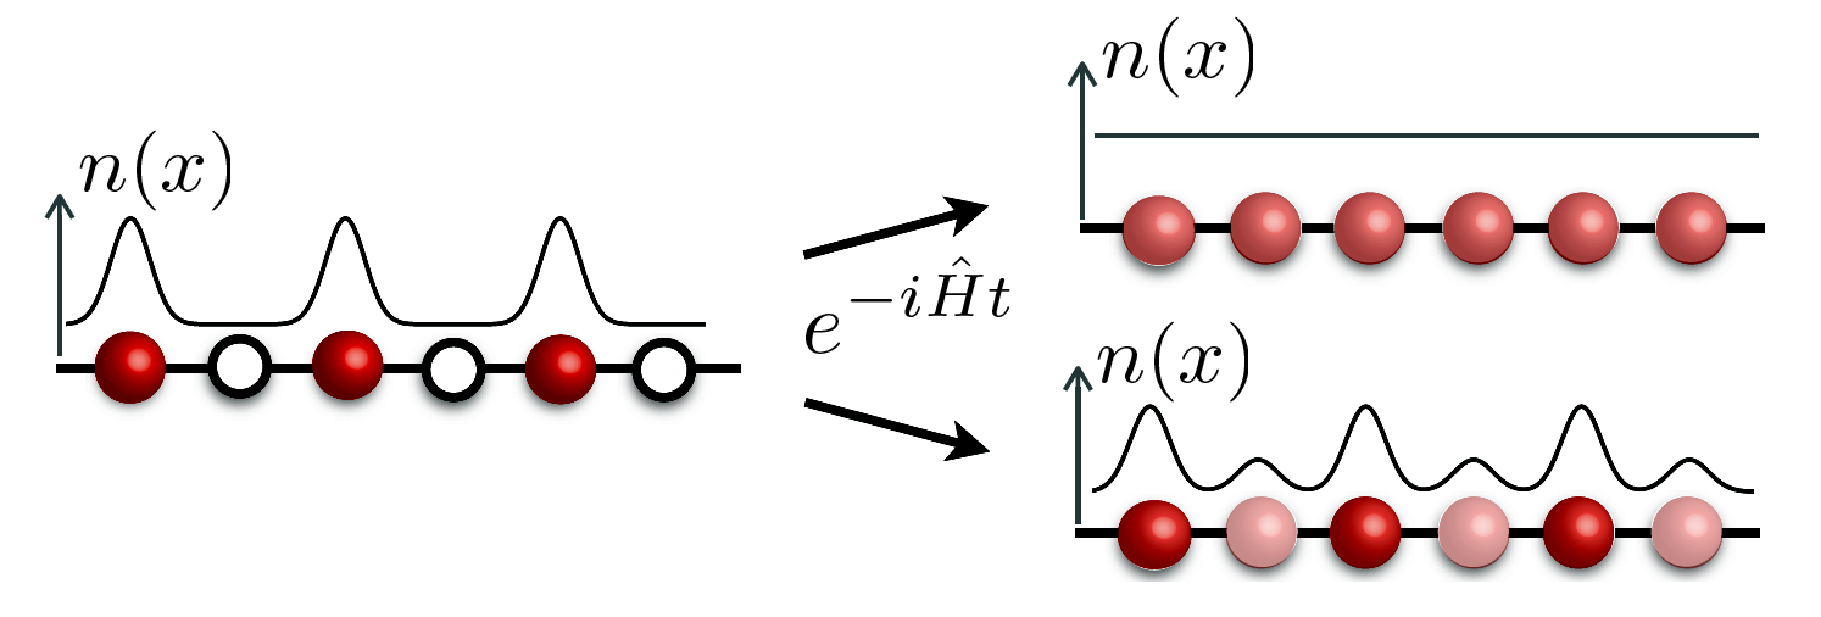
\includegraphics[width=1\textwidth]{abanin_thermalization_scheme.pdf}}
\caption{Shematski prikaz razlike med unitarnim časovnim razvojem netipične začetne konfiguracije interagirajočih delcev v ergodičnem in MBL režimu, kjer je netipičnost dosežena z alternirajočo zasedenostjo mest na kristalni verigi.
 V prvem primeru sistem sčasoma relaksira proti ravnovesni enakomerni porazdelitvi delcev, medtem ko se tovrstna relaksacija v MBL fazi ne zgodi. Slika je bila vzeta iz Ref.~\cite{abanin2018ergodicity}. }
\label{fig:abanin_thermalization}
\end{figure}
\end{minipage}
spoznanja teorije naključnih matrik~\cite{d2016quantum} (ang. \emph{random-matrix theory}, v nadaljevanju RMT), v okviru katere so podane teoretične napovedi~\cite{atas2013distribution} za vrednosti različnih spektralnih statistik in opazljivk, s katerimi primerjam svoje izračune. Slednji temeljijo na statistični obdelavi spektrov, dobljenih z eksaktno diagonalizacijo modelskih hamiltonk. \\\\
Uvodoma vpeljem in predstavim model t-J z dodanim potencialnim neredom kot značilen primer večdelčne hamiltonke, primerne za analizo prehoda med ergodično in MBL fazo. Nato podrobneje opišem dve izmed možnih spektralnih statistik, porazdelitev sosednjih energijskih nivojev in povprečno razmerje sosednjih razmikov med nivoji, ter razložim njuno numerično implementacijo. Sledita predstavitev rezultatov in diskusija. 

% \section{Reševanje naloge}
\section{Model t-J}
V zaključni nalogi kot primeren modelski sistem obravnavam model t-J~\cite{spalek2007tj} s periodičnimi robnimi pogoji na enodimenzionalni verigi, ki ga v okviru približka tesne vezi podaja hamiltonka 
\begin{equation}\label{eq:tJ_ham}
\begin{split}
\hat{H}&=-t\sum\limits_{i, \sigma} \left(\tilde{c}_{i,\sigma}^\dagger\tilde{c}_{i+1,\sigma} + c.c. \right) + J\sum\limits_i \left(S_i\cdot S_{i+1} - \frac{n_i n_{i+1}}{4}\right) + \sum\limits_i w_iS_i^z + \sum\limits_{i,\sigma} h_i n_{i,\sigma}=  \\
&=
H_t + H_J + H_w + H_h.
\end{split}
\end{equation} 
Pri tem so $\tilde{c}_{i,\sigma}^\dagger$ in  $\tilde{c}_{i,\sigma}$ \emph{projicirani} fermionski kreacijski in anihilacijski operatorji, ki jih vpeljemo v skladu s predpisom 
\begin{equation}
\tilde{c}_{i,\sigma}^\dagger=c_{i,\sigma}^\dagger(1-n_{i,-\sigma}) \hspace{5mm}\tilde{c}_{i,\sigma}=(1-n_{i,-\sigma})c_{i,\sigma}.
\end{equation}
Tako definirani kreacijski operatorji lahko na $i$-tem mestu v kristalni verigi ustvarijo delec z dano $z$-projekcijo spina $\sigma$ samo v primeru, ko se na mestu predhodno še ne nahaja delec z nasprotno projekcijo spina na os $z$. Na ta način preprečimo dvojno fermionsko zasedenost mest, člen $H_t$ v hamiltonki pa predstavlja skakanje (ang. \emph{hopping}) nosilcev naboja s tuneliranjem  med sosednjimi mesti na verigi, kjer je $t$ verjetnost za tovrstno tuneliranje. Zaradi enostavnosti obravnavamo samo skakanje med najbližjimi sosedi. \\\\ 
Pri zapisu zgornje hamiltonke upoštevamo t.i. \emph{bazo zasedenosti posameznih mest} (ang. \emph{site-occupational basis}), kjer so na $i$-tem mestu v kristalni rešetki možna tri stanja, in sicer 
$$
\ket{\psi_{i_0}}=\ket{0}_i, \hspace{5mm} \ket{\psi_{i_1}}=\ket{\uparrow}_i,\hspace{5mm} \ket{\psi_{i_{-1}}}=\ket{\downarrow}_i.
$$
V prvem stanju na $i$-tem mestu ni elektrona oziroma se tam nahaja vrzel, preostali dve stanji pa ustrezata prisotnosti elektrona s spinom $1/2$ in eno izmed dveh možnih projekcih spina na os $z$, medtem ko je dvojna zasedenost mesta prepovedana.  \\\\
Meddelčno interakcijo v hamiltonki modelira Heisenbergov izmenjalni člen $H_J$, kjer so $S_i$ spinski operatorji za spin $1/2$ in velja $S_i\cdot S_{j}=\frac{1}{2}\left(S_i^+S_j^- + S_i^-S_j^+\right) + S_i^zS_j^z$. Pri tem $J$ podaja velikost izmenjalne interakcije, kjer za slednjo v nalogi vselej privzamem izotropijo. Delovanje členov $H_t$ in $H_J$ je shematsko prikazano in razloženo na Sliki \ref{fig:tJ_scheme}. \\\\
S členom $H_w$ v hamiltonki modeliram prispevek naključnega magnetnega polja v smeri osi $z$, ki se zeemansko sklaplja s 
spinskimi prostostnimi stopnjami, pri čemer je $w_i$ velikost naključno izžrebanega magnetnega polja na $i$-tem mestu v kristalni rešetki. Podobno člen $H_h$ modelira potencialni nered, ki se sklaplja z vrzelmi v kristalni rešetki, $h_i$ pa je naključno izžrebana vrednost energije vrzeli, ki se nahaja na $i$-tem mestu v kristalni rešetki. Vrednosti $w_i$ in $h_i$ tipično izžrebam v skladu s škatlasto verjetnostno porazdelitvijo, kot prikazuje Slika \ref{fig:prob_dist}, na kateri sta $W$ in $H$	 parametra 
nereda, s katerima določam velikost spinskega in vrzelnega potencialnega nereda. Prehod med ergodično in MBL fazo
v modelu zasledujem kot funkcijo velikosti obeh omenjenih parametrov.
\begin{minipage}[t]{0.35\textwidth}
\noindent
 \\\\ 
 V nalogi uporabljam za velikost sistema oznako $L$, z $N_h$ označujem število vrzeli, z $N_u$ pa število spinov $1/2$ s projekcijo spina navzgor. Pri analizi se vselej osredotočim na podprostor hamiltonke, podane z En. \eqref{eq:tJ_ham}, s fiksnim številom vrzeli in ničelno skupno projekcijo spina na os $z$, $S^z=0$. Stanja z ničelno skupno projekcijo spina so v hamiltonki najštevilčnejša in se pojavljajo v vseh spinskih blokih, zato gre za statistično najbolj zastopan sektor. Število stanj v podprostoru s fiksnim številom vrzeli in ničelnim spinom določimo s pomočjo kombinatorike - najprej prešteje{}mo število razporeditev $N_h$ vrzeli na $L$ mest v verigi, kar nato pomnožimo še s številom razporeditev $N_u$ spinov na preostalih $L-N_h$ mest. Število stanj torej podaja zveza
\begin{equation}\label{eq:nstat}
N_\mathrm{stat}=\binom{L}{N_j}\binom{L-N_h}{N_u},
\end{equation}
kar je za različna števila vrzeli in različne velikosti sistemov grafično prikazano na Sliki~\ref{fig:tJ_num_states}.
\end{minipage}\hfill
\begin{minipage}[t]{0.6\textwidth}
\begin{figure}[H]
\centering{
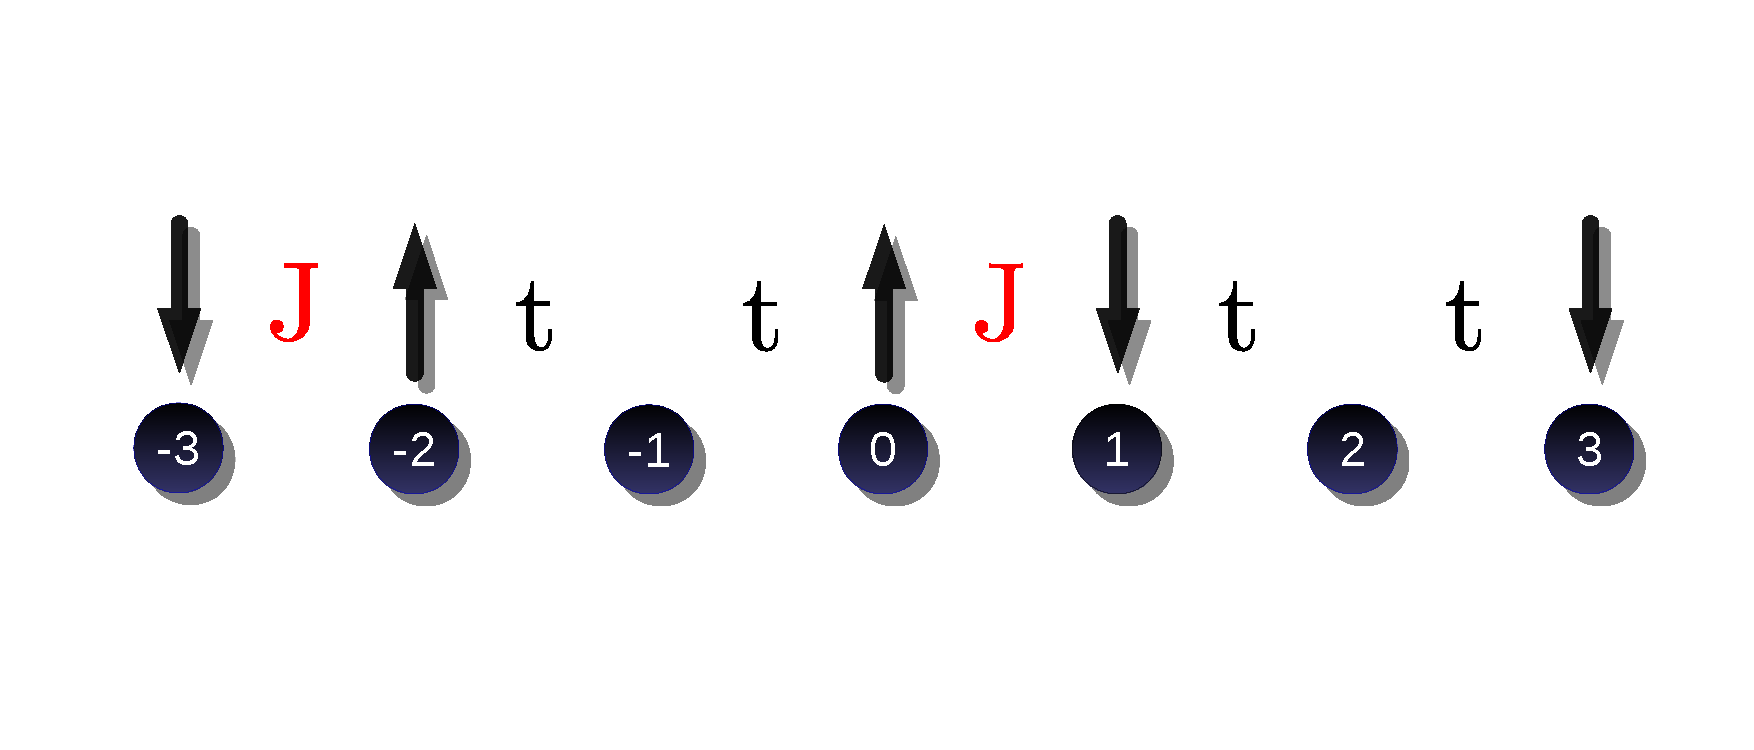
\includegraphics[width=0.8\textwidth]{tJ_scheme.pdf}}
\caption{Shematski prikaz modela t-J na verigi z $L=7$ mesti, $N_h=2$ vrzelma in $N_u=2$ navzgor obrnjenima spinoma in odprtimi robnimi pogoji.	 $J$ označuje velikost izmenjalne interakcije med spini sosednjih elektronov, ki obrne par nasprotno obrnjenih spinov (ang. \emph{spin-flips}). Verjetnost za tuneliranje elektrona na prazno mesto označuje $t$. }
\label{fig:tJ_scheme}
\end{figure}
\begin{figure}[H]
\centering{
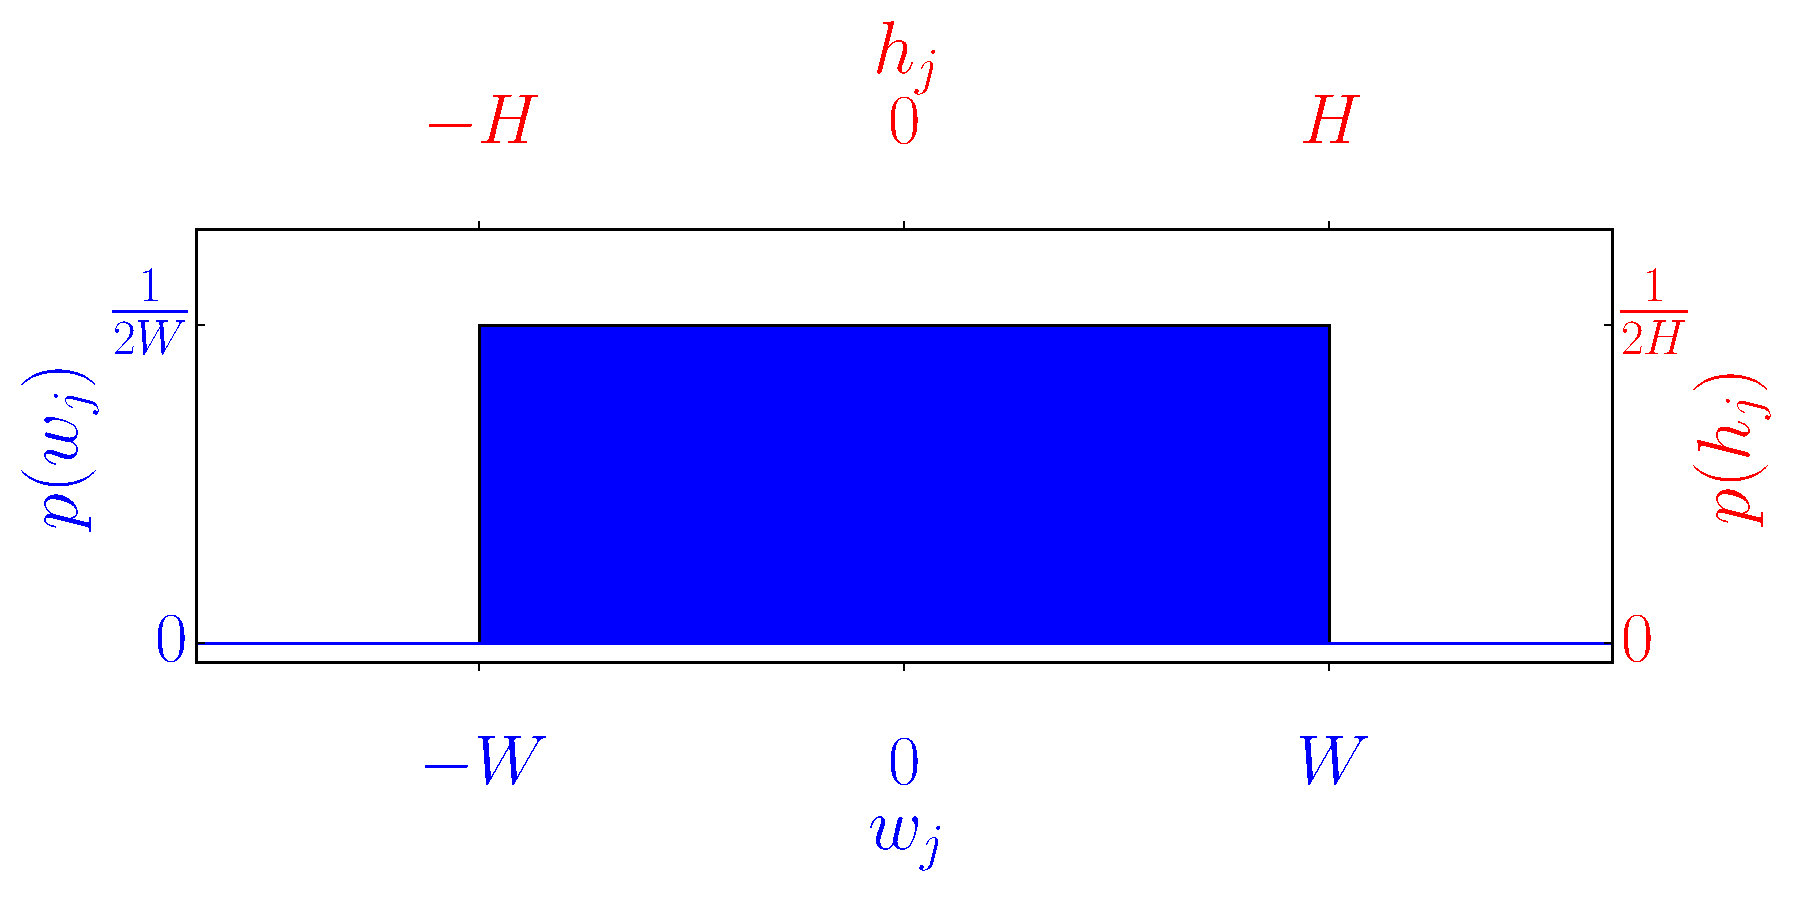
\includegraphics[width=0.8\textwidth]{prob_dist.pdf}}
\caption{Naključne vrednosti magnetnega polja $w_i$ in potenciala $h_i$ tipično izžrebam v skladu s škatlasto verjetnostno porazdelitvijo, kjer sta $W$ in $H$ parametra nereda. Varianca takšne porazdelitve je enaka $\frac{A^2}{3}$, kjer je $A$ eden izmed obeh parametrov nereda.  }
\label{fig:prob_dist}
\end{figure}

\end{minipage}

% \begin{figure}[H]
% \floatbox[{\capbeside\thisfloatsetup{capbesideposition={left,center},capbesidewidth=6cm}}]{figure}[\FBwidth]
% {\caption{Naključne vrednosti magnetnega polja $w_i$ in potenciala $h_i$ tipično izžrebam v skladu s škatlasto verjetnostjo porazdelitvijo, kjer sta $W$ in $H$ parametra nereda. }\label{fig:prob_dist}}
% {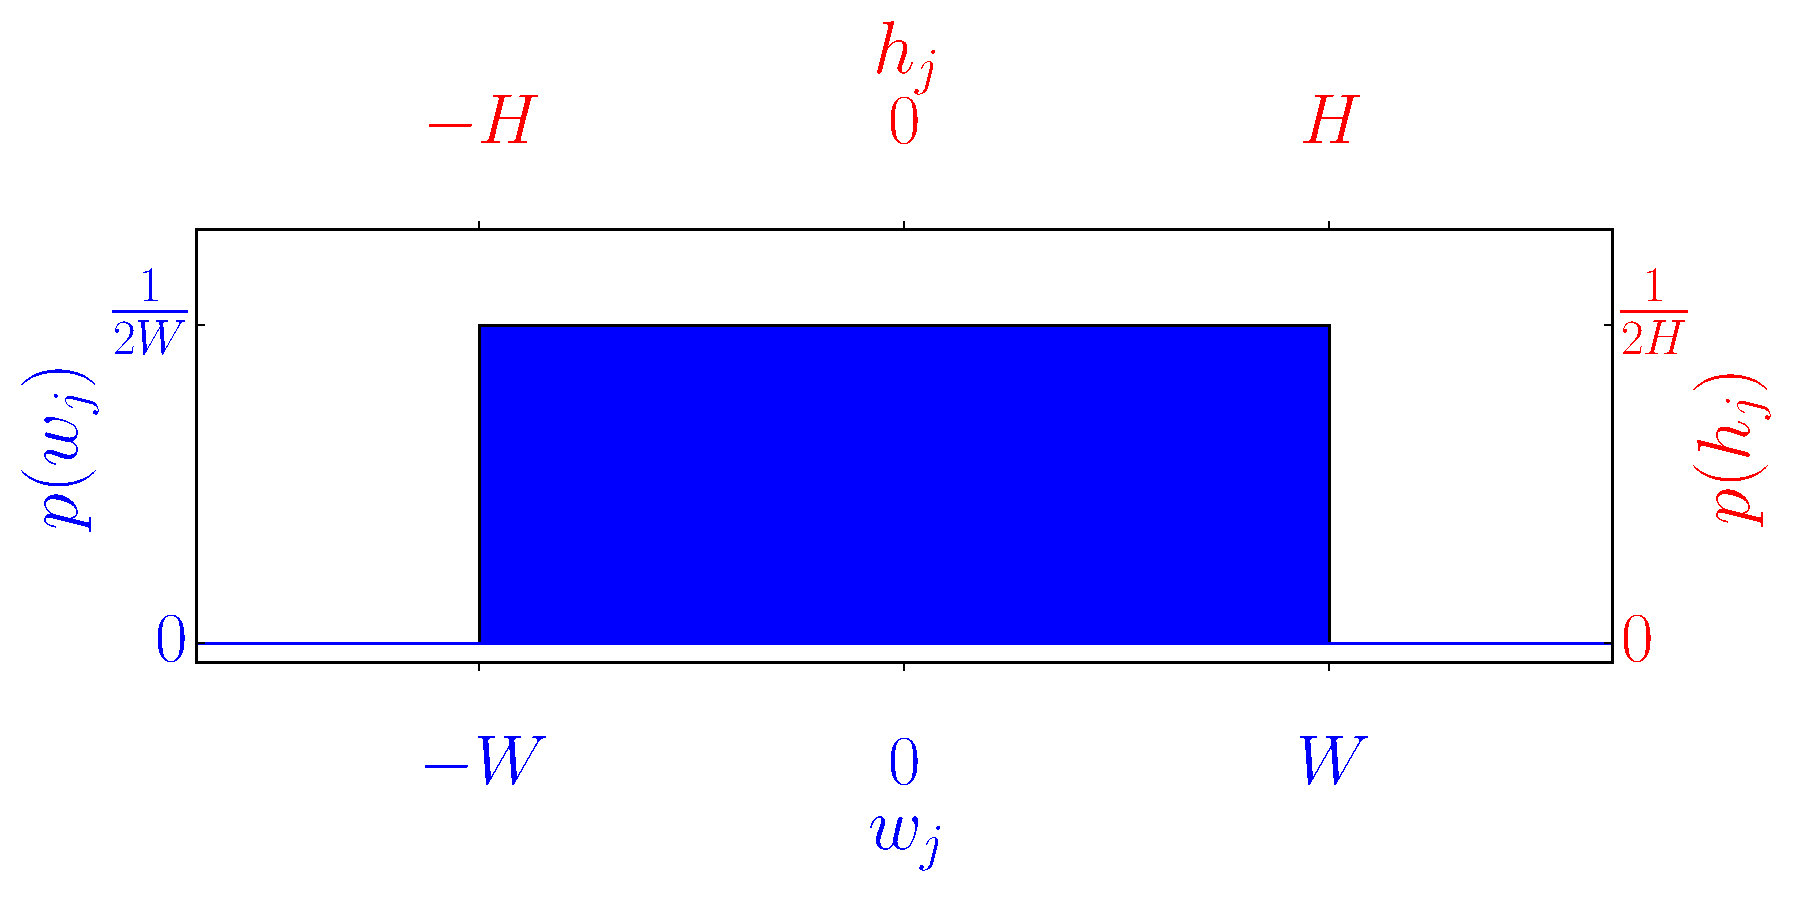
\includegraphics[width=0.62\textwidth]{prob_dist.pdf}}
% \end{figure}

\begin{figure}[H]
\floatbox[{\capbeside\thisfloatsetup{capbesideposition={left,center},capbesidewidth=6cm}}]{figure}[\FBwidth]
{\caption{Odvisnost števila stanj od velikosti sistema in števila dopantov (vrzeli) razkrije, da smo pri študijah s polno diagonalizacijo precej omejeni s številom dostopnih sistemov, ki so nam na voljo, kar precej oteži skalirno analizo, s katero bi radi napovedali obnašanje sistema v termodinamski limiti neskončnega sistema. }\label{fig:tJ_num_states}}
{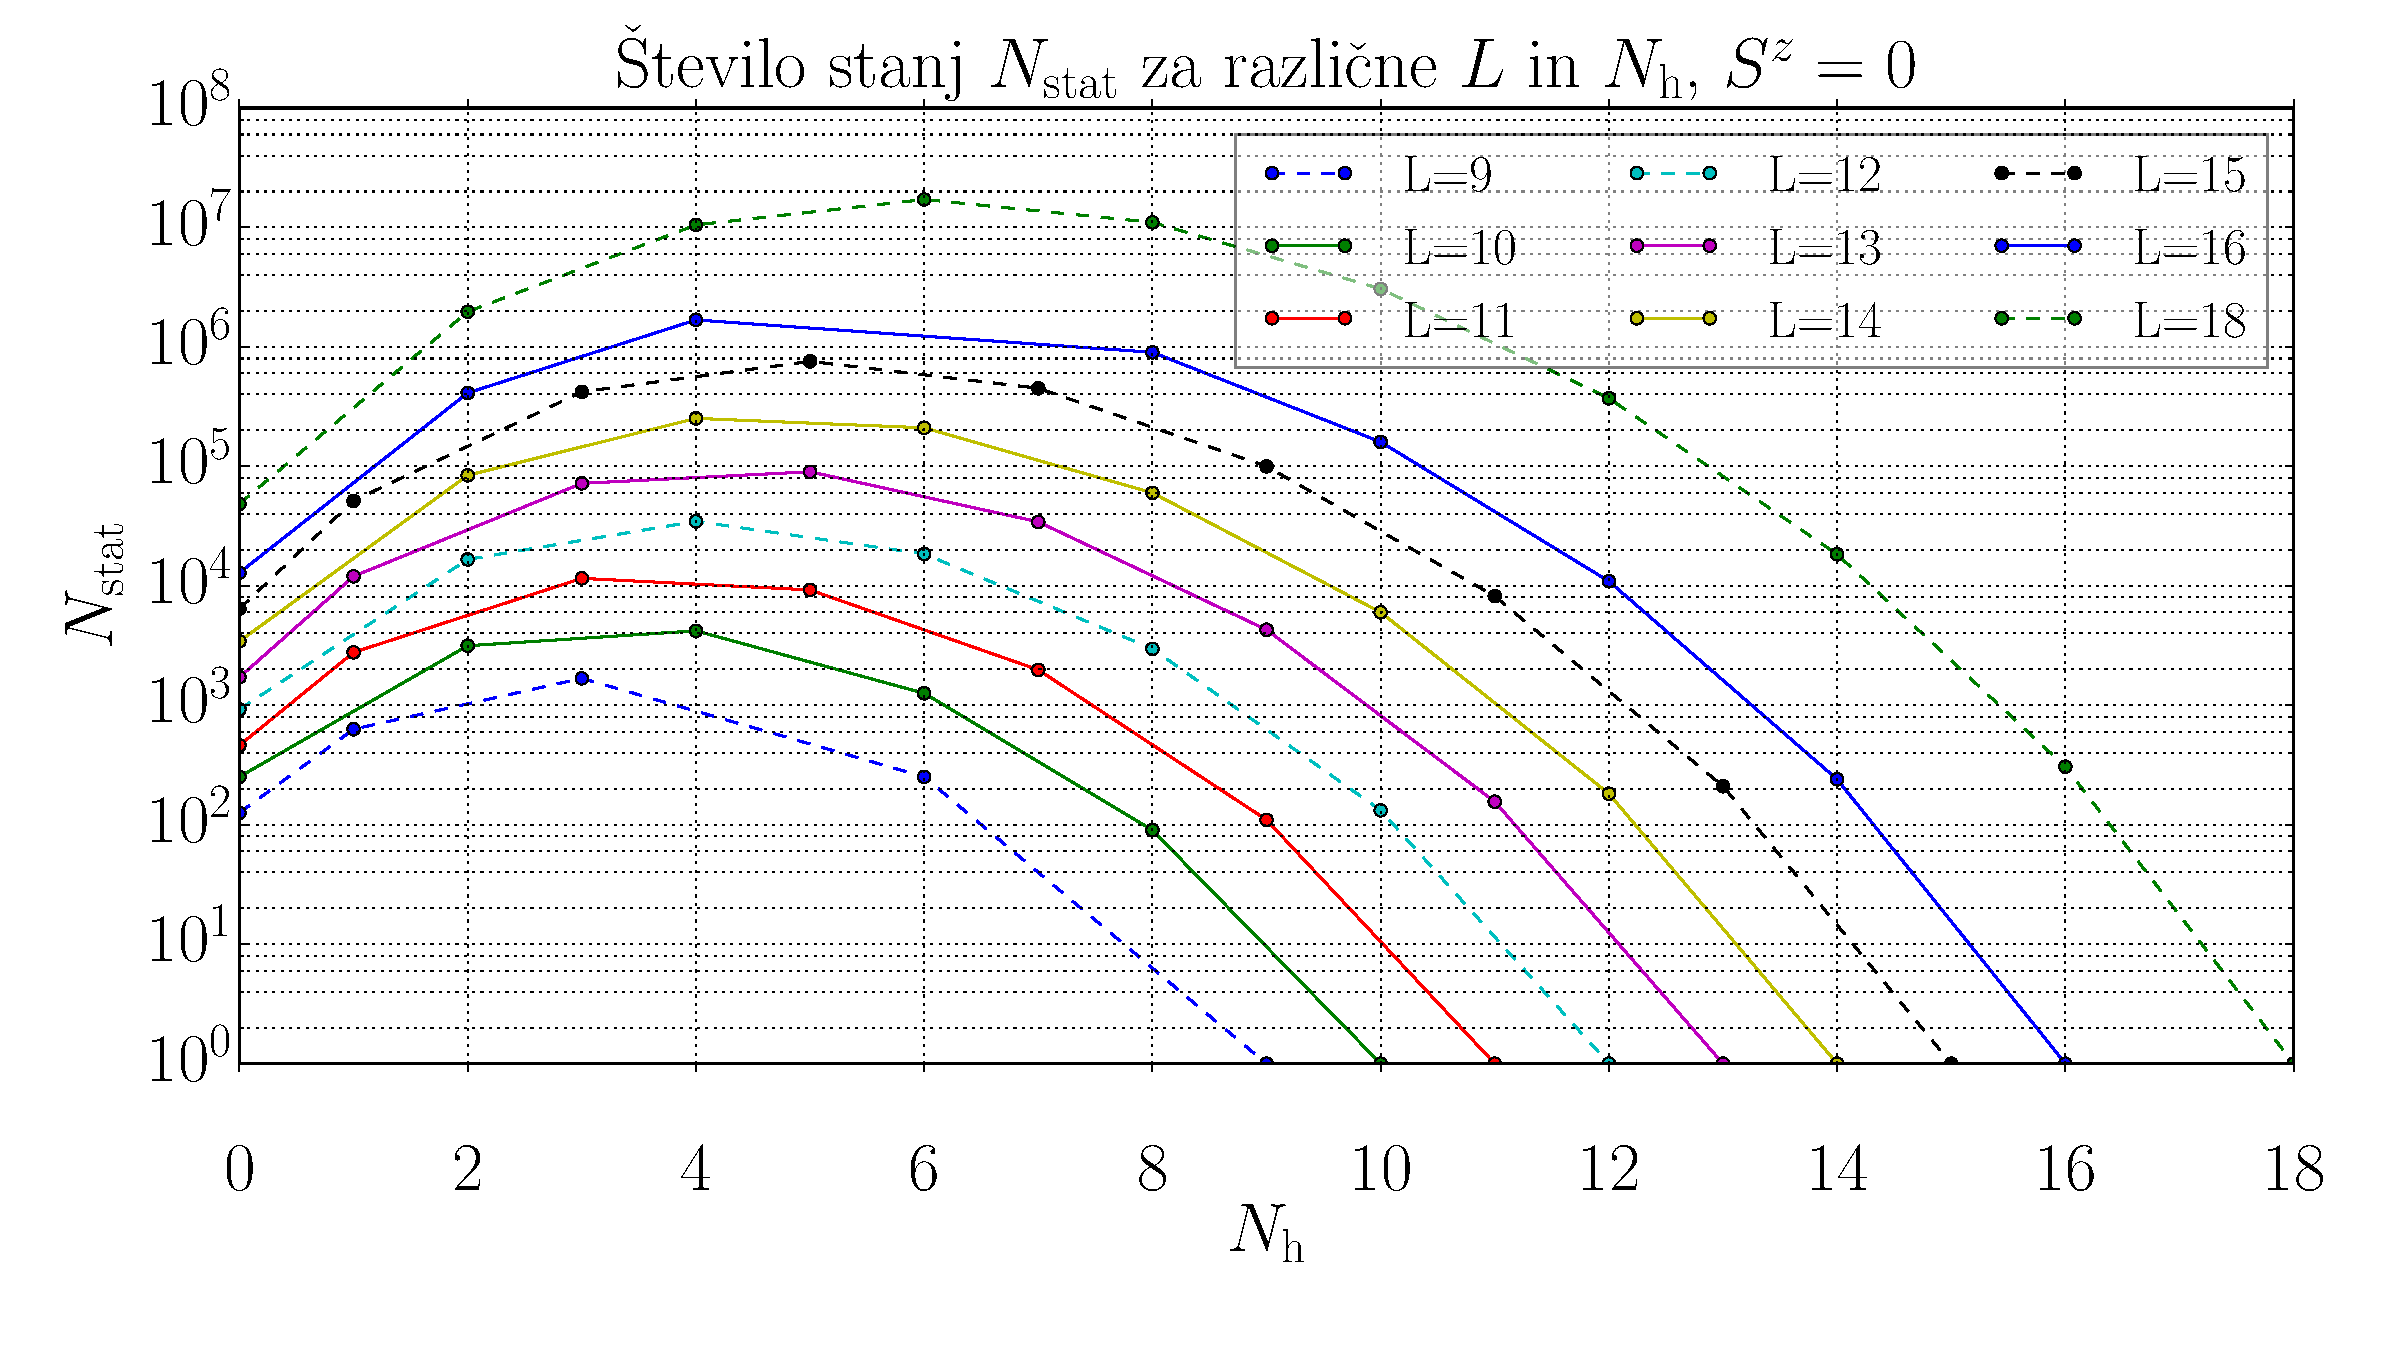
\includegraphics[width=0.62\textwidth]{tJ_num_states.pdf}}
\end{figure}
% \subsubsection{Numerična implementacija modela}
Za potrebe zaključne naloge sem se omejil na sisteme z največ 34650 ($L=12$, $N_h=4$, $N_u=4$) stanji. Vsakokrat sem izžrebal med 100 in 300 različnih realizacij naključnega nereda, s katerimi sem pripravil hamiltonko, podano z En. \eqref{eq:tJ_ham}. Končne rezultate, ki so predstavljeni v nadaljevanju naloge, sem dobil s povprečenjem rezultatov po različnih realizacijah nereda. Prehod med ergodičnim in MBL režimom me je zanimal kot funkcija velikosti parametrov nereda $W$ in $H$. V odsotnosti vsakršnega nereda je pričakovano ergodično obnašanje sistema, zanimalo pa me je, ali lahko dodajanje nereda vodi do prehoda v MBL fazo. Brez predolgih izletov v teorijo lokalizacije v kvantnih sistemih lahko pričakovanja deloma upraviči predpostavka, da povečevanje nereda v sistemu povečuje vpliv diagonalnih členov v hamiltonki, podani z En. \eqref{eq:tJ_ham}, v primerjavi z izvendiagonalnimi členi, ki omogočajo prenos spina in nabojev med mesti na kristalni verigi in tako pripomorejo k ergodični relaksaciji netipičnih začetnih konfiguracij stanj.  
\section{Statistika sosednjih energijskih nivojev}
Za presojo ergodičnosti oziroma večdelčne lokaliziranosti sistema analiziram statistiko energijskih spektrov modelske hamiltonke pri različnih vrednostih parametrov nereda $W$ in $H$. Pri tem s pridom izkoriščam spoznanja teorije naključnih matrik~\cite{mehta2004random} (RMT), ki temelji na pionirskem delu Eugenea Wignerja in Freemana J. Dysona, ki sta razvila teoretični model za opis energijskih spektrov kompleksnih atomskih jeder. Njuna ideja temelji na predpostavki, da je točna napoved energijskih nivojev in njim pripadajočih lastnih stanj v kompleksnih sistemih, kot so jedra težkih elementov, tako rekoč brezupna naloga. Namesto točnega izračuna je zato smiselneje preučevati statistične lastnosti spektrov. Druga ključna opazka je, da imajo modelske hamiltonke kompleksnih sistemov v generičnih bazah strukturo, ki je močno podobna strukturi naključnih matrik. Slednje velja v primeru, ko matrične elemente opazujemo v dovolj ozkem energijskem oknu, v katerem je gostota stanj približno konstantna. Analiza spektralnih lastnosti naključnih matrik tako lahko omogoči vpogled tudi v spektralne lastnosti hamiltonk kompleksnih sistemov, v kolikor zagotovimo, da naključne matrike pripadajo simetrijskemu razredu preučevane modelske hamiltonke. \\

 Generičnost baze pomeni splošno izbiro baze, ki ni posebej `prikrojena' za potrebe našega problema. V predhodnem poglavju predstavljena baza zasedenosti stanj ali baza lastnih stanj hamiltonke seveda nista generični bazi, saj ima v njih hamiltonka redko pasovno oziroma diagonalno strukturo, neničelni matrični elementi pa so vse prej kot naključni~\cite{d2016quantum}. Napovedi RMT so kljub temu veljavne, saj predpostavka naključnih matričnih elementov velja za izbiro splošne baze. \\\\
 V podpoglavjih, ki sledita, predstavim Wigner-Dysonovo in Poissonovo statistiko, ki opišeta razmik med sosednjimi energijskimi nivoji v ergodičnem in MBL ali integrabilnem sistemu. Razmik med sosednjimi energijskimi nivoji je definiran kot 
 \begin{equation}\label{eq:razmik}
 s_n=E_{n+1}-E_n,
 \end{equation}
 kjer je $E_n$ $n$-ti energijski nivo. \\\\
 Poleg statistike odmikov med sosednjimi nivoji 
 preučujem tudi statistiko razmerij odmikov med sosednjimi energijskimi nivoji, ki sta jo v članku iz leta 2007~\cite{PhysRevB.75.155111} prva uvedla Oganesyan in Huse:
 \begin{equation}\label{eq:oganesyan_huse}
 \tilde{r}_n=\frac{\min\left(s_n,s_{n-1}\right)}{\max\left(s_n,s_{n-1}\right)}, \hspace{5mm} r_n=\frac{s_n}{s_{n-1}}.
 \end{equation}
 V praksi ergodičnost oziroma večdelčno lokaliziranost sistema presojam na podlagi povprečne vrednosti $\langle \tilde{r}\rangle$, za katero v obeh režimih obstajata dobro določeni limitni vrednosti~\cite{atas2013distribution}. Poleg tega je povprečje $\langle \tilde{r}\rangle$ za vizualizacijo prikladnejša količina kot porazdelitev energijskih nivojev. 
 \subsection{Wigner-Dysonova statistika razmikov med sosednjimi nivoji} 
 V tem podpoglavju izpeljem Wigner-Dysonovo statistiko za razmik med sosednjimi energijskimi nivoji v naključnih matrikah. Pri izpeljavi sledim preglednemu članku navedenem v Ref.~\cite{abanin2018ergodicity}. Osnovno idejo RMT lahko predstavimo z analizo hamiltonke velikosti $2\times2$, v kateri matrične elemente izžrebamo v skladu z Gaussovo verjetnostno porazdelitvijo z ničelnim povprečjem in varianco $\sigma$.  Pri tem upoštevamo še simetrije našega problema:
 \begin{equation}\label{eq:rnd_ham}
 \hat{H}=
 \begin{bmatrix}
 \varepsilon_1 & \frac{V}{\sqrt{2}} \\
 \frac{V^*}{\sqrt{2}} & \varepsilon_2
 \end{bmatrix}
 \end{equation}
 Če velja simetrija na obrat časa, $V=V^*$, lahko hamiltonko zapišemo kot realno matriko. Slednje drži tudi v primeru hamiltonke, podane z En. \eqref{eq:tJ_ham}. Diagonalizacija naključne $2\times2$ hamiltonke je enostavna, lastni energiji sta
 \begin{equation}
 E_{1,2}=\frac{\varepsilon_1+\varepsilon_2}{2}\pm \frac{1}{2}\sqrt{\left(\varepsilon_1 +\varepsilon_2\right)^2 + 2V^2}
 \end{equation}
 Od tod lahko izračunamo statistiko razmikov med energijskimi nivoji, $P(E_1-E_2=s)\equiv P(s),$
\begin{equation}
 P(s)=\frac{1}{\left(2\pi\right)^{3/2}\sigma^3}\int \dd\varepsilon_1\int\dd\varepsilon_2\int \dd V \delta\left(\sqrt{\left(\varepsilon_1 +\varepsilon_2\right)^2 + 2V^2}-s\right)\exp\left( -\frac{\varepsilon_1^2+\varepsilon_2^2+V^2}{2\sigma^2}\right)
 \end{equation}
 Z zamenjavo spremenljivk, $\varepsilon_2=\varepsilon_1+\sqrt{2}\xi$ in integracijo po $\varepsilon_1$ dobimo 
 \begin{equation}
 P(s)=\frac{1}{2\pi\sigma^2}\int\int\dd\xi\dd V\delta\left(\sqrt{2\xi^2+2V^2}\right)\exp\left(-\frac{\xi^2+V^2}{2\sigma^2}\right)
 \end{equation}
 Z uvedbo cilindričnih koordinat, $V=r\cos(x)$, $\xi=r\sin(x),$ dobimo 
 \begin{equation}\label{eq:wigner_surmise}
 P(s)=\frac{s}{2\sigma^2}\exp\left(-\frac{s^2}{4\sigma^2} \right)
\end{equation}
 Nazadnje porazdelitev še normirano in povprečni razmik med nivoji $\bar{s}$ postavimo na vrednost 1, pa dobimo za realne simetrične naključne matrike \emph{Wigner-Dysonovo} statistiko za razmik med energijskimi nivoji: 
 \begin{equation}\label{eq:wigner-dyson}
 P_\mathrm{WD}(s)=\frac{\pi s}{2}\exp\left(-\frac{\pi}{4}s^2\right)
 \end{equation}
 Zgornja statistika izkazuje dve splošni generični lastnosti, značilni za nivojske statistike kvantnih kaotičnih sistemov. V limiti $s\to 0$ je verjetnost za ničeln razmik med nivoji ničelna, kar kaže na odboj med nivoji (ang. \emph{level repulsion}). Kot bomo videli nekoliko kasneje, je to bistveno drugače od nivojskih statistik v integrabilnem ali MBL primeru. Za velike razmike $s$ verjetnost $P_\mathrm{WD}(s)$ pada kot gaussovska porazdelitev. Lastnosti statistike so bile sprva izpeljane za kvantne sisteme s klasičnim kaotičnim analogom, a se je kasneje izkazalo, da veljajo tudi za sisteme brez omenjene analogije.\\


 Izraz \eqref{eq:wigner_surmise} je eksakten za hamiltonke velikosti $2\times2$, izkaže pa se~\cite{abanin2018ergodicity}~\cite{atas2013distribution}, da je ujemanje dobro tudi za višjedimezionalne hamiltonke. V tem primeru definiramo ansambel naključnih matrik, ki jih žrebamo v skladu z naključno Gaussovsko porazdelitvijo kot
 \begin{equation}
 P_\mathrm{GOE}(\hat{H})\propto \exp\left(-\frac{1}{2a^2}\Tr\left(\hat{H}^2\right) \right) \equiv \exp\left(-\frac{1}{2a^2}\sum\limits_{ij}H_{ij}H_{ji} \right)
 \end{equation}
 Tako definiran ansambel matrik se imenuje gaussovski ortogonalni ansambel (GOE), z zgornjo definicijo pa zadostimo zahtevi po invariantnosti ansambla na vsakršne ortogonalne transformacije, saj je porazdelitev odvisna zgolj od sledi kvadrata posamezne hamiltonke, kar je po definiciji invariantna količina. Hkrati je porazdelitev gaussovska, saj je sled vsota kvadratov naključno porazdeljenih matričnih elementov in kot takšna zadošča centralnemu limitnemu izreku. \\\\Izpeljava natančnih izrazov za nivojske statistike hamiltonk iz GOE ni predmet te zaključne naloge, v splošnem zanje zaključena analitična oblika niti ne obstaja. Podrobnejša analiza je navedena v članku v Ref.~\cite{atas2013distribution}, tu bom za presojo uporabljal rezultat, podan z En. \eqref{eq:wigner_surmise}, ki dobro popiše tudi večdimenzionalne primere. 
 \subsection{Poissonova statistika razmikov med sosednjimi nivoji}
 V predhodnem podpoglavju smo obravnavali nivojsko statistiko v kvantnokaotičnih sistemih, v katerih so razmiki med sosednjimi energijskimi nivoji porazdeljeni v skladu z Wigner-Dysonovo statistiko. Porazdelitev za kvantne integrabilne sisteme sta prva obravnavala Berry in Tabor v članku iz leta 1977~\cite{berry1977level}. Za potrebe razjasnitve pojmov, ki nastopajo v zaključni nalogi, bom tu navedel zgolj ključne rezultate. \\\\
 Med enostavnejše primere neergodičnega sistema sodi veriga neodvisnih kvantnih harmonskih oscilatorjev z nesoizmerljivimi frekvencami. V odsotnosti medsebojne sklopitve lahko vsakega izmed oscilatorjev diagonaliziramo neodvisno od preostalih, skupno energijo pa dobimo s seštevanjem enooscilatorskih energij kot 
 $$
 E=\sum_j n_j\omega_j,
 $$ 
 kjer je $j$ lastna frekvenca, $n_j$ pa zasedbeno število $j$-tega oscilatorja. Za velike vrednosti $E$ dobimo podobne vrednosti energije za različne nabore zasedbenih števil $\{n_j\}$, zato lahko energijske nivoje obravnavamo kot nekorelirana naključna števila. V tem primeru je verjetnost, da se na energijskem intervalu dolžine $\delta E$ nahaja $m$ energijskih nivojev, enaka Poissonovi porazdelitvi 
 \begin{equation}
 P_m=\frac{\lambda^m}{m!}\exp\left(-\lambda \delta E\right),
 \end{equation}
 kjer je $\lambda$ enaka inverznemu povprečnemu razmiku med nivoji v spektru. Porazdelitev razmikov med nivoji tako dobimo na enak način kot porazdelitev čakalnih časov med dogodki v Poissonovem procesu:
 \begin{equation}\label{eq:poisson}
 P_\mathrm{Poisson}(s)=P_0=\exp\left(-s\right)
 \end{equation}
 Pri tem smo postavili $\lambda=1$ in vpeljali $s$ kot  $s=\delta E$. V nasprotju z Wigner-Dysonovo porazdelitvijo pri Poissonovi statistiki ni odboja med nivoji, saj ima porazdelitev vrh pri $s=0$. V integrabilnih sistemih je slednje posledica ohranjenih količin. Podobno je v MBL sistemih veljavnost Poissonove statistike posledica uvedbe naključnih členov v modelsko hamiltonko. \\\\
 Splošna izjava, ki povzame vsebino tega podpoglavja, pravi, da izkazujejo kvantni sistemi s klasičnim analogom Poissonovo statistiko razmikov med sosednjimi energijskimi nivoji. Izjava drži tudi v primeru mnogih kvantnih sistemov brez klasične ustreznice, kljub temu pa obstajajo tudi protiprimeri, npr. en delec v harmonskem potencialu. Predpostavka veljavnosti Poissonove statistike je zato danes znana kot \emph{domneva} Berrya in Taborja (ang. \emph{Berry-Tabor conjecture})~\cite{berry1977level}.\\\\
 Na Sliki \ref{fig:unfolding_demo_three_slo} so prikazani primeri numerično izračunanih nivojskih statistik v ergodičnem, vmesnem in MBL režimu skupaj z Wigner-Dysonovo in Poissonovo statistiko. 
 \subsection{Statistika razmerij odmikov sosednjih nivojev $\tilde{r}$}
 Po postopku, ki ga opišem v poglavju o numerični implementaciji izračunov, izračunam povprečno vrednost količine $\tilde{r}$, ki jo podaja En. \eqref{eq:oganesyan_huse}. V ergodičnem primeru mora izračunana vrednost $\langle \tilde{r}\rangle$ čim bolje ustrezati GOE vrednosti, ki znaša:
 \begin{equation}\label{eq:r_GOE}
 \langle \tilde{r}\rangle_\mathrm{GOE}=0.5307
 \end{equation}
 V integrabilnem ali MBL primeru ustreza povprečno razmerje razmikov sosednjih nivojev vrednosti za Poissonovo porazdeljen spekter lastnih vrednosti: 
 \begin{equation}\label{eq:r_poisson}
 \langle \tilde{r}\rangle_\mathrm{Poisson}=0.38629
 \end{equation}

\begin{figure}[H]
\centering{
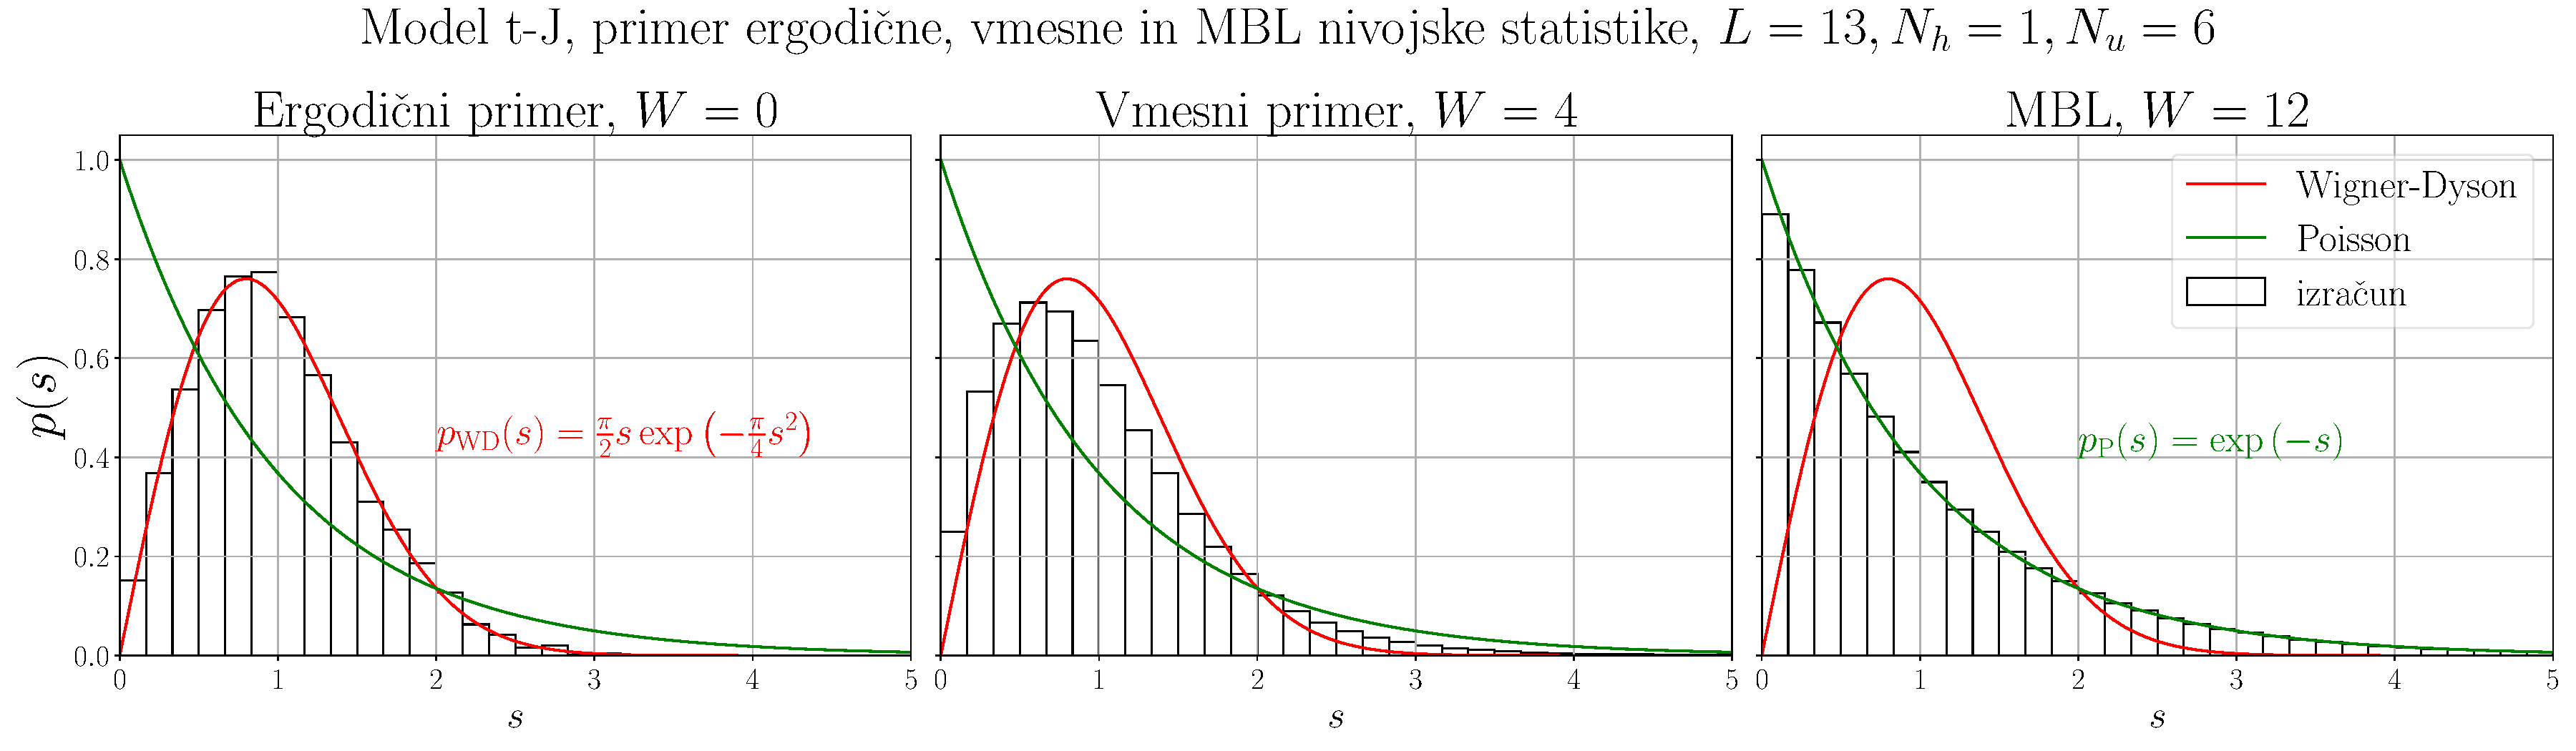
\includegraphics[width=1\textwidth]{unfolding_demo_three_slo.pdf}}
\caption{Numerično izračunana statistika razmikov med sosednjimi energijskimi nivoji za model t-J, $L=13$, $N_h=1$, $N_u=6$. Na podlagi komplementarnih študij časovne dinamike modela~\cite{lemut2017complete} sem izbral vrednosti parametra spinskega nereda $W$, za katere je obnašanje sistema poznano. Pri $W=0$ je sistem ergodičen, kar je razvidno iz ujemanja numeričnih izračunov s krivuljo Wigner-Dysonove statistike, podobno je pri $W=12$ dobro ujemanje s krivuljo Poissonove statistike. V vmesnem režimu se numerično izračunane vrednosti ne ujemajo z nobeno od teoretičnih napovedi. Pri dani konfiguraciji ima model 12012 stanj, rezultate pa sem dobil s povprečenjem po 100 realizacijah spinskega nereda. Natančne podrobnosti numerične implementacije so podane v naslednjem poglavju.  }
\label{fig:unfolding_demo_three_slo}
\end{figure}

\begin{figure}[H]
\centering{
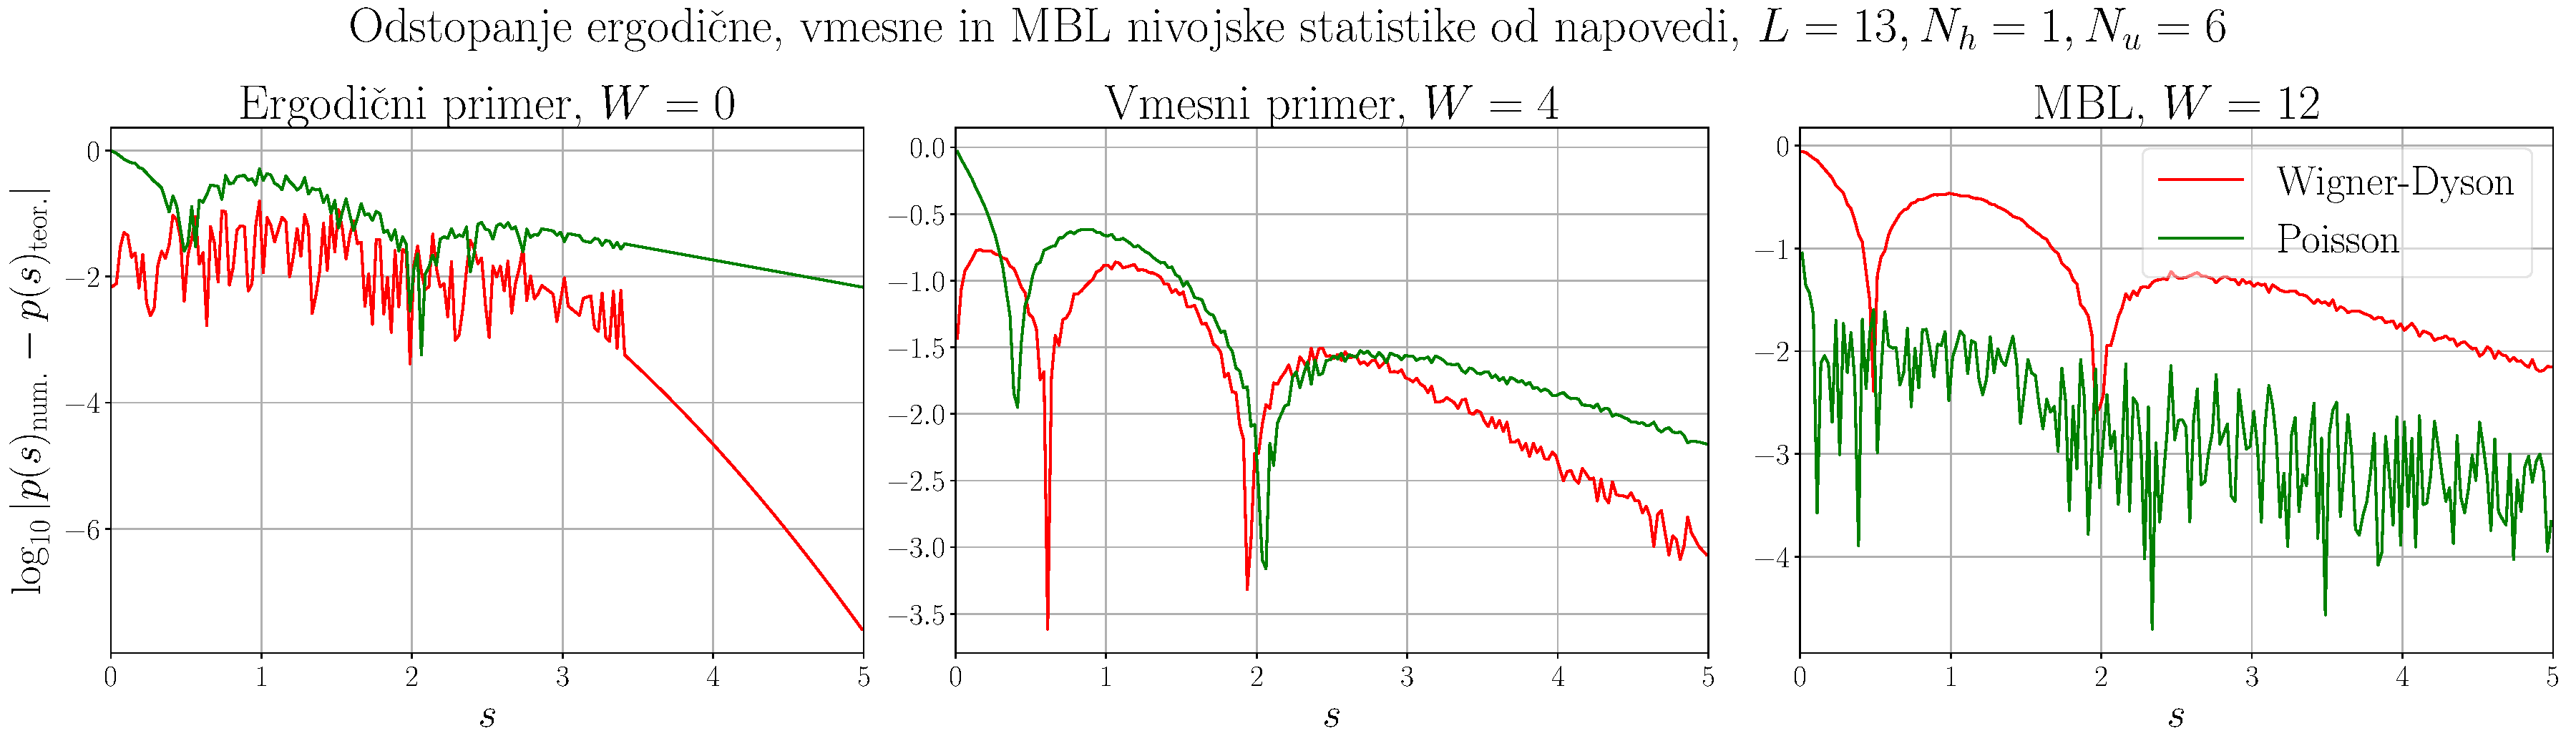
\includegraphics[width=1\textwidth]{unfolding_demo_three_error_slo.pdf}}
\caption{Desetiški logaritem absolutne vrednosti razlike med numerično vrednostjo in teoretično napovedjo za primere izračunov, predstavljene na Sliki~\ref{fig:unfolding_demo_three_slo}. Vsakokrat sta za primerjavo predstavljena izračuna za Wigner-Dysonovo in Poissonovo statistiko. }
\label{fig:unfolding_demo_three_error_slo}
\end{figure}
% \subsubsection{Test ujemanja numeričnih vrednosti s teoretičnimi napovedmi z uporabo testa Kolmogorova in Smirnova}
% Ujemanje numeričnih rezultatov, prikazanih na Slikah~\ref{fig:unfolding_demo_three_slo} in~\ref{fig:unfolding_demo_three_error_slo}, s teoretičnimi napovedmi sem preveril še z uporabo testa Kolmogorova in Smirnova. Za Wigner-Dysonovo porazdelitev, podano z En. \eqref{eq:wigner-dyson}, znaša kumulativna porazdelitev 
% \begin{equation}
% \mathrm{CDF}_\mathrm{WD}(s)=1 - \exp\left(\frac{-\pi s^2}{4}\right).
% \end{equation}
% Za Poissonovo porazdelitev, podano z En.~\eqref{eq:poisson}, znaša kumulativna porazdelitev
% \begin{equation}
% \mathrm{CDF}_\mathrm{Poisson}(s)=1-\exp\left(-s \right).
% \end{equation}
% Pri izračunih sem uporabil vgrajeno funkcijo \url{stats.kstest()} iz paketa \url{scipy.stats}.
 \section{Numerična implementacija in rezultati}
 Za izračun spektralne statistike hamiltonko, podano z En. \eqref{eq:tJ_ham}, pri danih vrednostih parametrov $t, J, W$ in $H$ najprej diagonaliziram pri različnih realizacijah nereda. Za diagonalizacijo uporabim program, napisan v programskem jeziku \url{fortran}, pri čemer diagonalizacijo izvedem z rutino \url{spev} iz Intelove knjižnice \url{MKL}, ki je namenjena diagonalizaciji realnih simetričnih matrik. Izračune izvajam na gruči \url{LIPS} na odseku F1 na Inštitutu Jožef Stefan. Primer rezultatov diagonalizacije je prikazan na grafih na Slikah~\ref{fig:Eigenstates_spin_hole_disorder_13_1_6.pdf} in~\ref{fig:Eigenstates_spin_hole_disorder_12_4_4.pdf}, in sicer za primera z dopiranjem z eno vrzeljo in s tretjinskim dopiranjem. Grafi na Slikah~\ref{fig:Eigenstates_spin_hole_disorder_13_1_6.pdf} in~\ref{fig:DOS_spin_hole_disorder_12_4_4.pdf} prikazujejo normalizirano gostoto stanj za oba primera. 	
 \begin{figure}[H]
\centering{
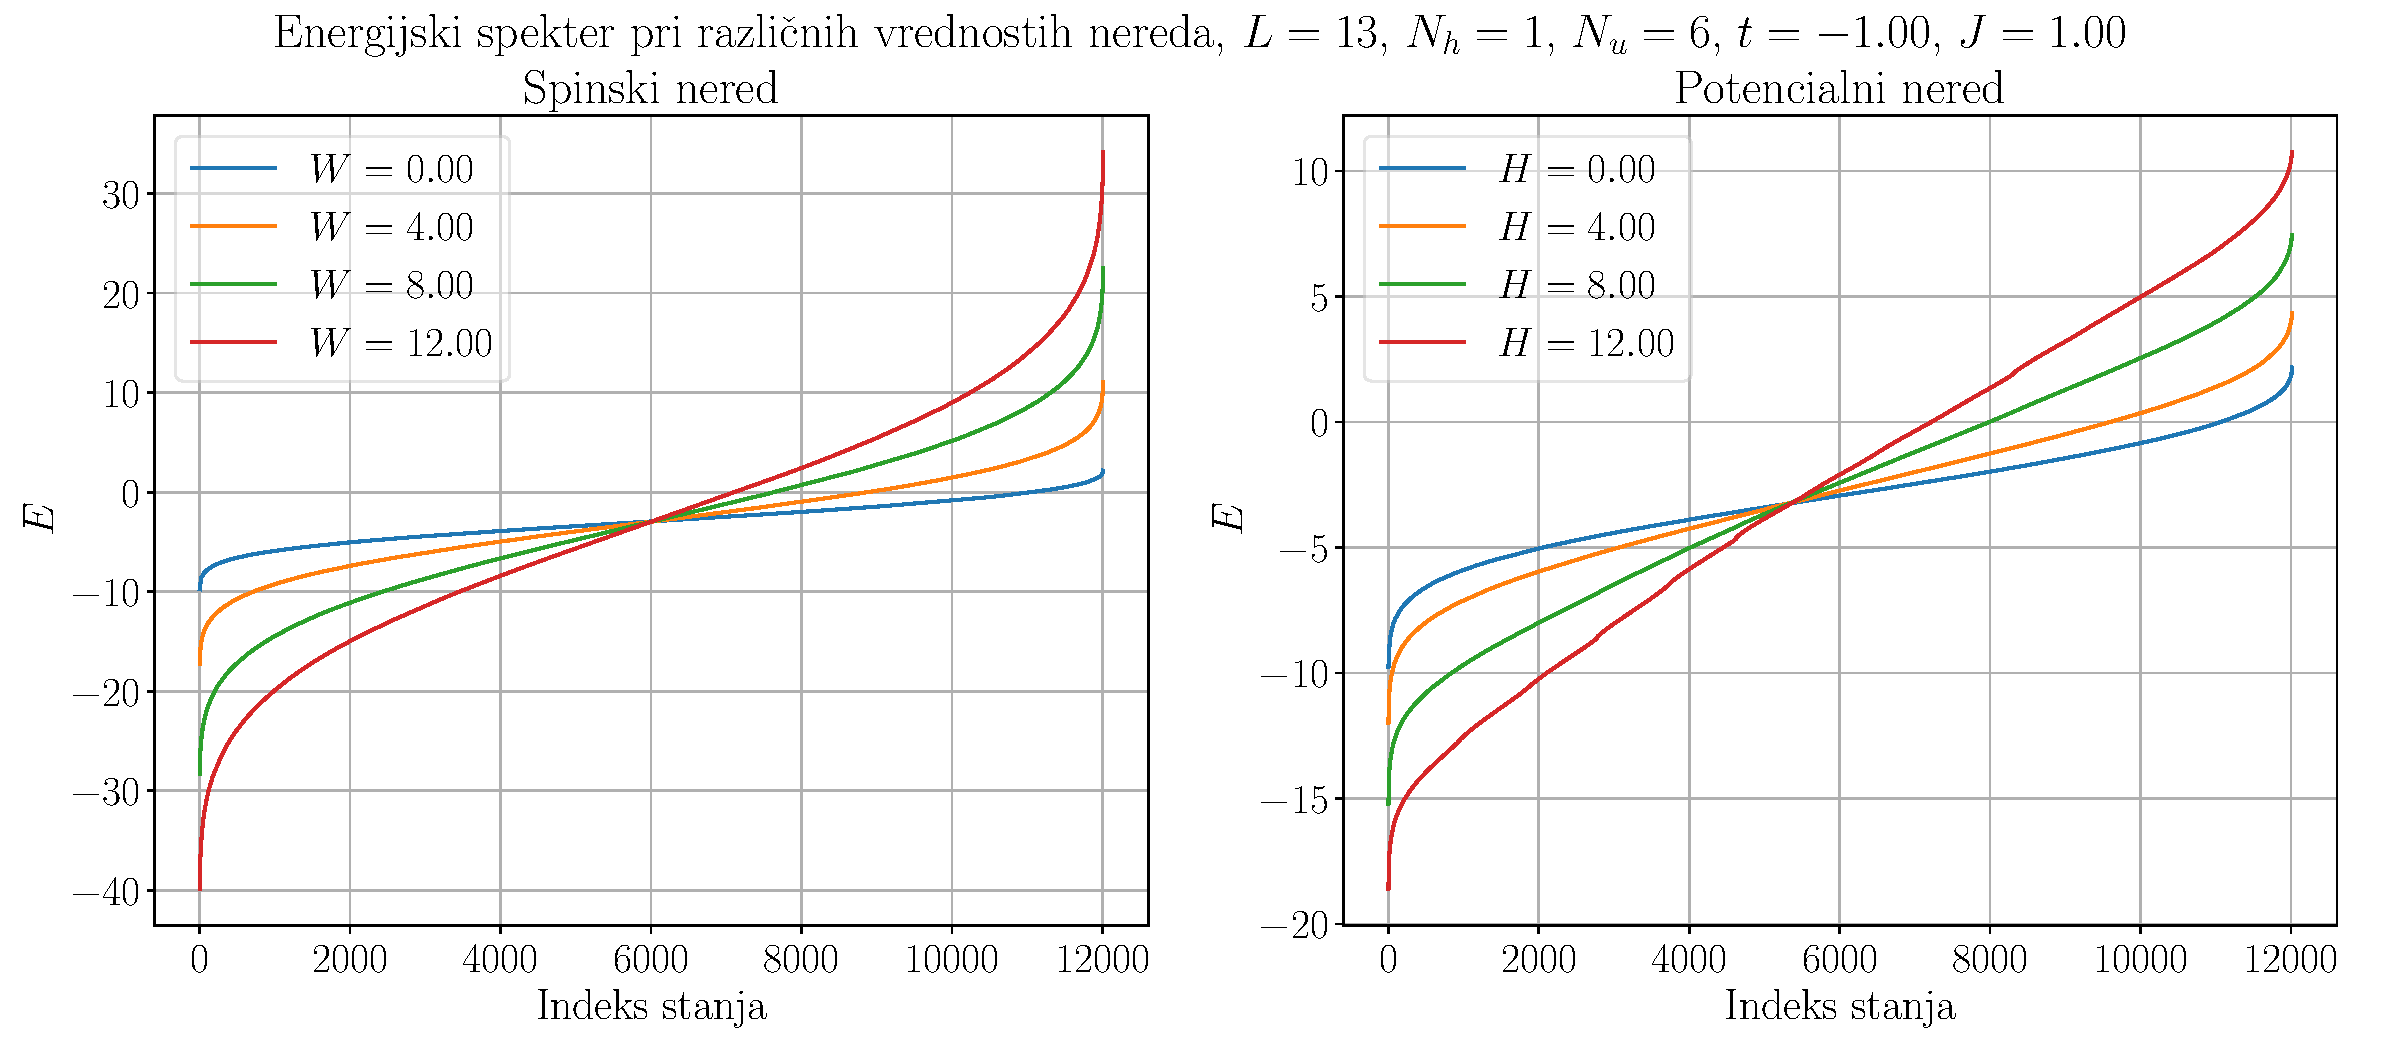
\includegraphics[width=1\textwidth]{Eigenstates_spin_hole_disorder_13_1_6.pdf}}
\caption{Primeri energijskih spektrov pri $L=13, N_h=1, N_u=6.$ Prikazani so rezultati za različne vrednosti parametrov $W$ in $H$, pri čemer sem rezultate za spinski nered vsakokrat dobil s povprečenjem po 100 realizacijah nereda, rezultate za potencialni nered pa s povprečenjem po 600 realizacijah. Pri dopiranju z eno samo vrzeljo opazimo, da je vpliv povečevanja spinskega nereda na spekter znatno večji od vpliva povečevanja potencialnega nereda. Razlog povprečenja po večjem številu realizacijah spinskega nereda je naveden v komentarju k Sliki~\ref{fig:DOS_spin_hole_disorder_13_1_6.pdf}.  }
\label{fig:Eigenstates_spin_hole_disorder_13_1_6.pdf}
\end{figure}
 \begin{figure}[H]
\centering{
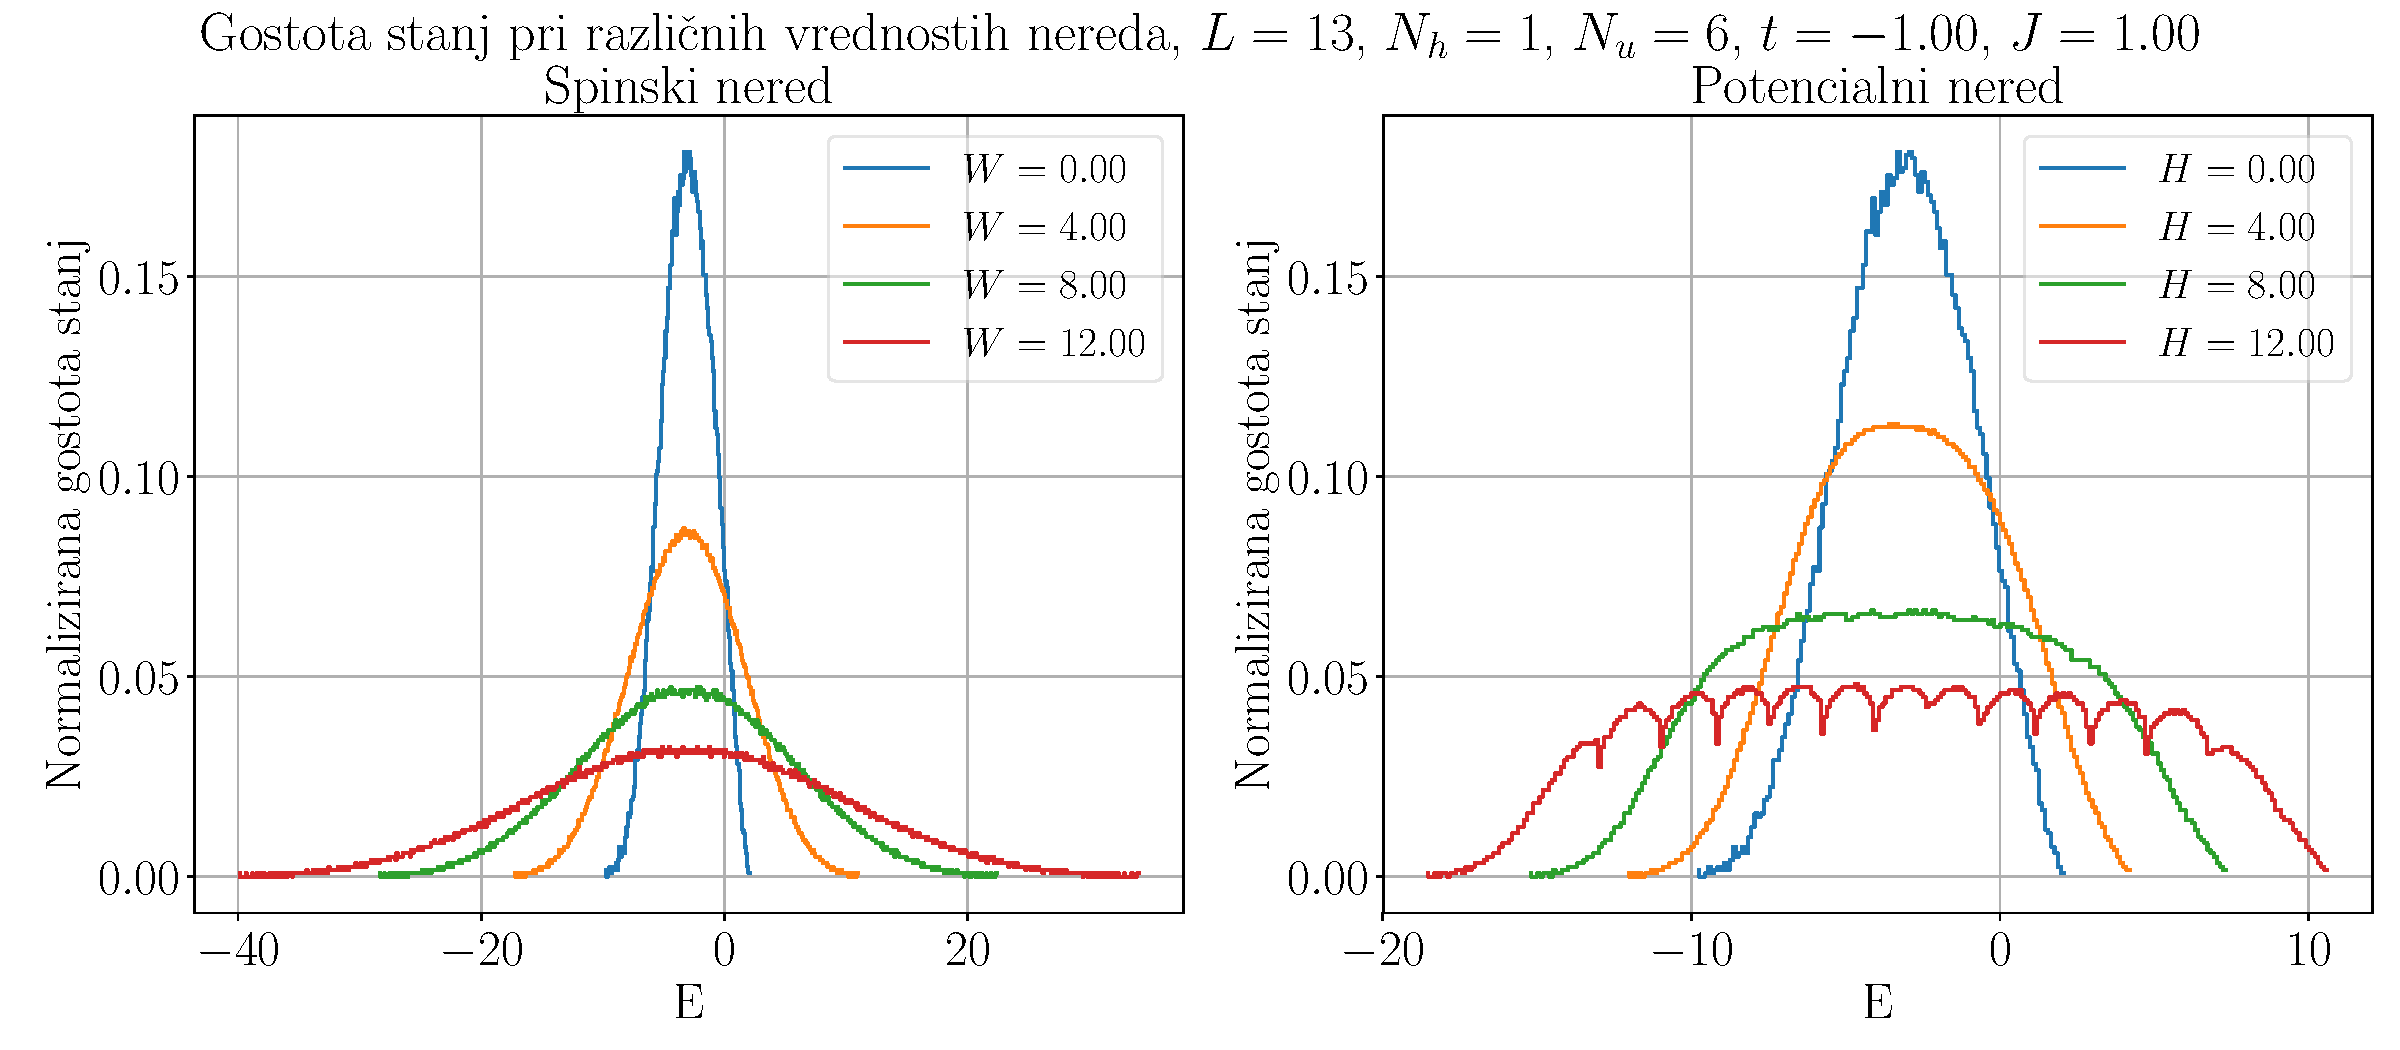
\includegraphics[width=0.9\textwidth]{DOS_spin_hole_disorder_13_1_6.pdf}}
\caption{Normalizirano število stanj na energijski interval za spektre, prikazane na Sliki~\ref{fig:Eigenstates_spin_hole_disorder_13_1_6.pdf}. V primeru spinskega nereda ima gostota stanj vselej izrazit vrh na sredini spektra. Oscilacije v primeru velikega potencialnega nereda $H=12.00$ so najverjetneje posledica prisotnosti zgolj ene vrzeli. Slednjo lahko na $L$ mest razporedimo na $L$ načinov, toliko je tudi različnih matričnih elementov v (diagonalnem) naključnem potencialnem členu $\hat{H}_h$. Glede na naključno potencialno energijo so vse spinske konfiguracije pri danem položaju vrzeli medsebojno degenerirane z degeneracijo enako $N_\mathrm{stat}/L$. Pri velikih parametrih nereda $H$, kot je na naši energijski skali npr. $H=12.00$, postane prispevek člena $\hat{H}_h$ v hamiltonki dominanten, zato (najverjetneje) opazimo oscilacije gostote stanj. Lokalni minimumi slednje ločijo ravno $L=13$ različnih sektorjev. Grafe za spinski nered sem dobil s povprečenjem po 100 realizacijah nereda, grafe za potencialni nered pa s povprečenjem po 600 realizacijah. Zanimalo me je, kakšna je pri potencialnem neredu vloga povprečenja, saj sem oscilacije gostote stanj najprej razumel kot nekakšen statistični artefakt. Kvalitativno se ne zdi, da bi večje povprečenje bistveno spremenilo obliko krivulje, zato v poročilo vključujem samo primer povprečenja po 600 vzorcih.}
\label{fig:DOS_spin_hole_disorder_13_1_6.pdf}
\end{figure}
 \begin{figure}[H]
\centering{
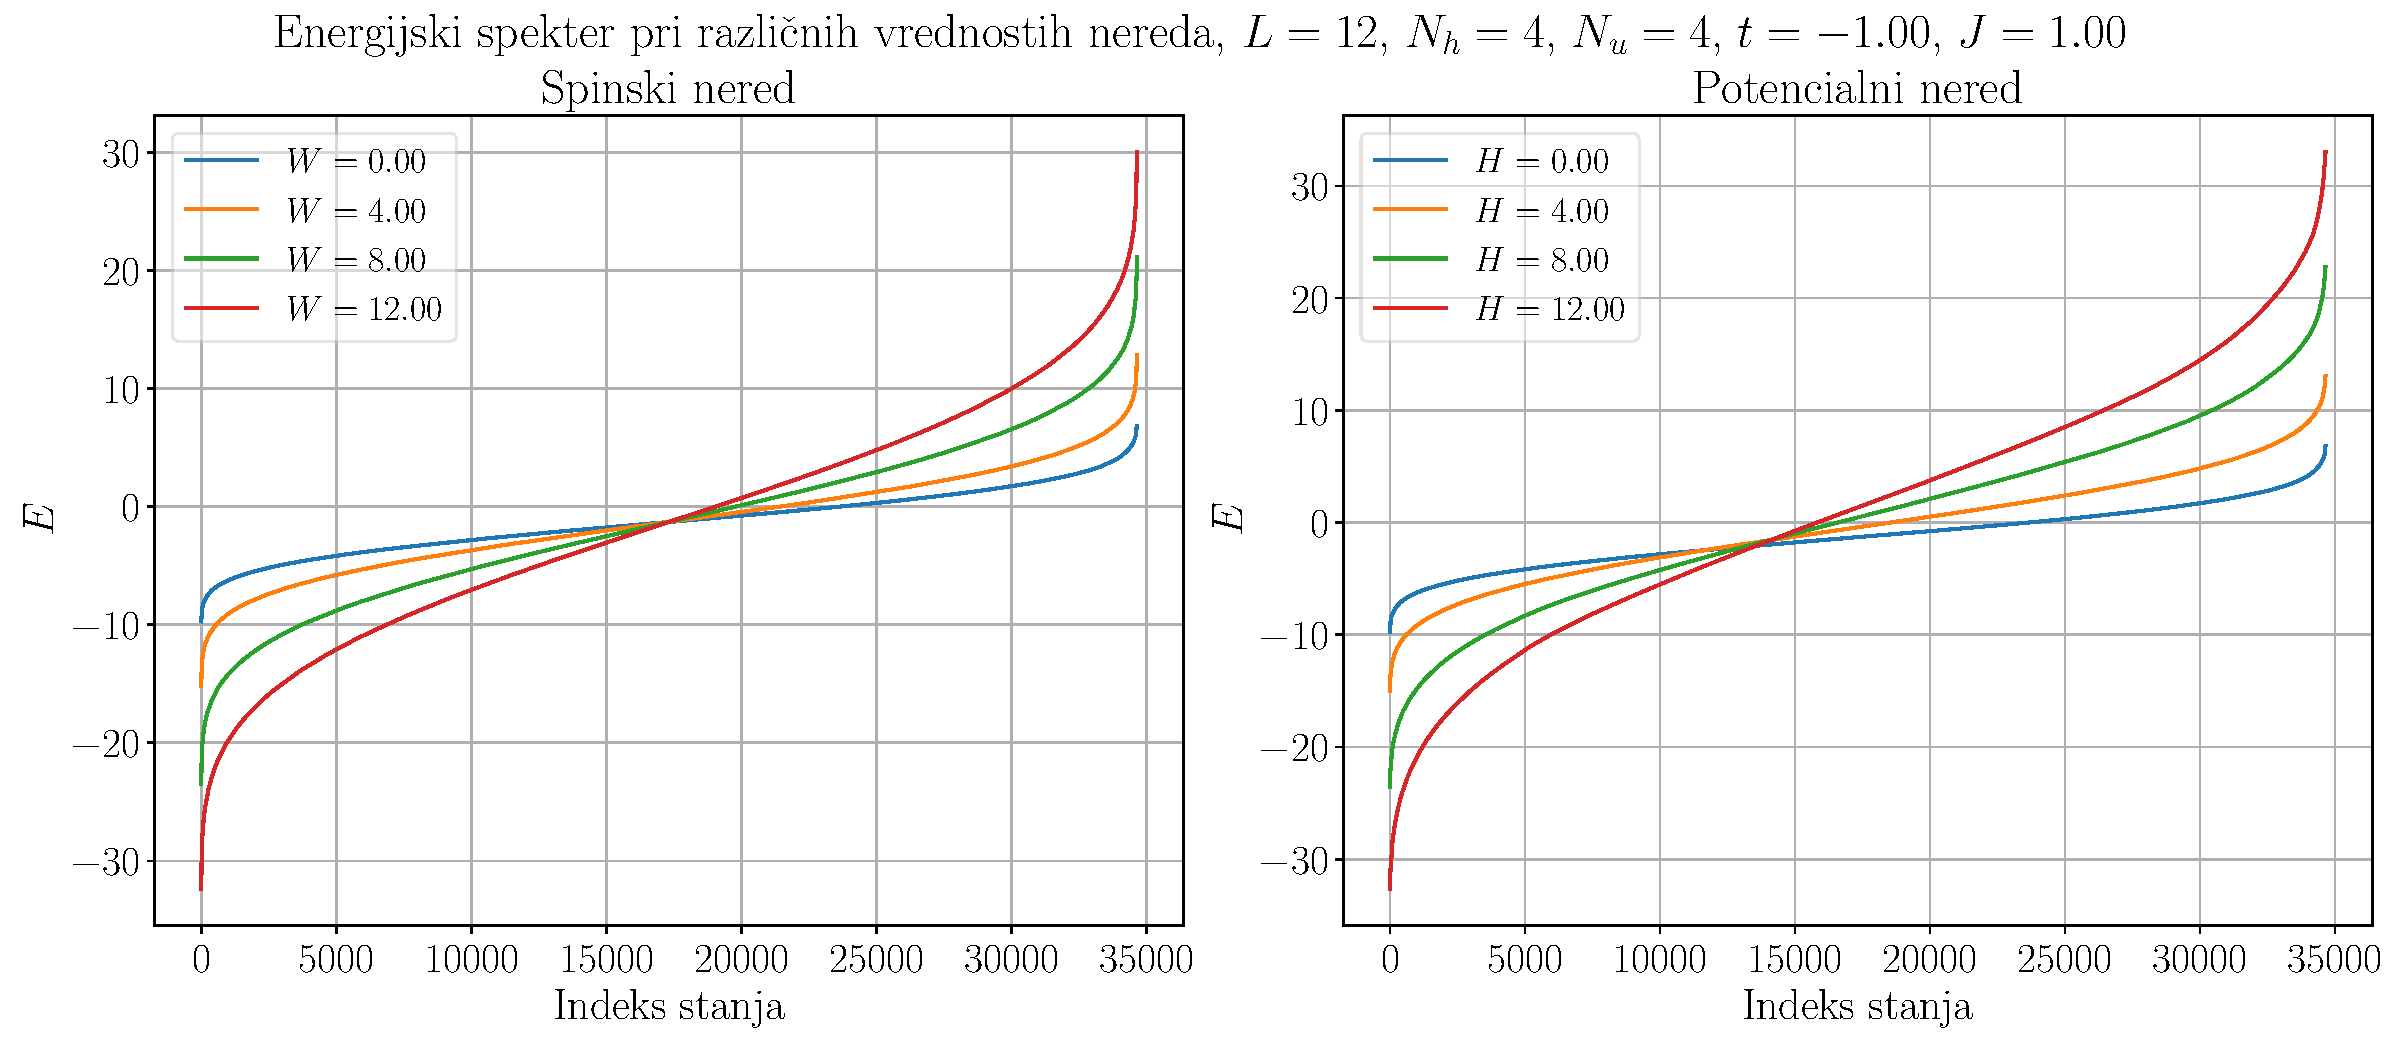
\includegraphics[width=1\textwidth]{Eigenstates_spin_hole_disorder_12_4_4.pdf}}
\caption{Energijski spektri v primeru spinskega in potencialnega nereda za tretjinsko dopiranje na sistemu z $N_\mathrm{stat}=34650$ stanji. V tem primeru sta vpliva spinskega in potencialnega nereda na širino spektra dokaj podobna. Energijsko skalo prispevka spinskega nereda ocenimo kot $(L-n_h)\cdot \frac{W}{2}$, kjer s faktorjem $\frac{1}{2}$ upoštevam velikost spina v izrazu za zeemansko sklopitev spinov z magnetnim poljem. Energijsko skalo potencialnega nereda podaja vrednost $n_h\cdot H$. Zaradi razmeroma velikih sistemov sem povprečenje izvedel po $50$ naključnih vzorcih za vsak tip nereda.   }
\label{fig:Eigenstates_spin_hole_disorder_12_4_4.pdf}
\end{figure}
 \begin{figure}[H]
\centering{
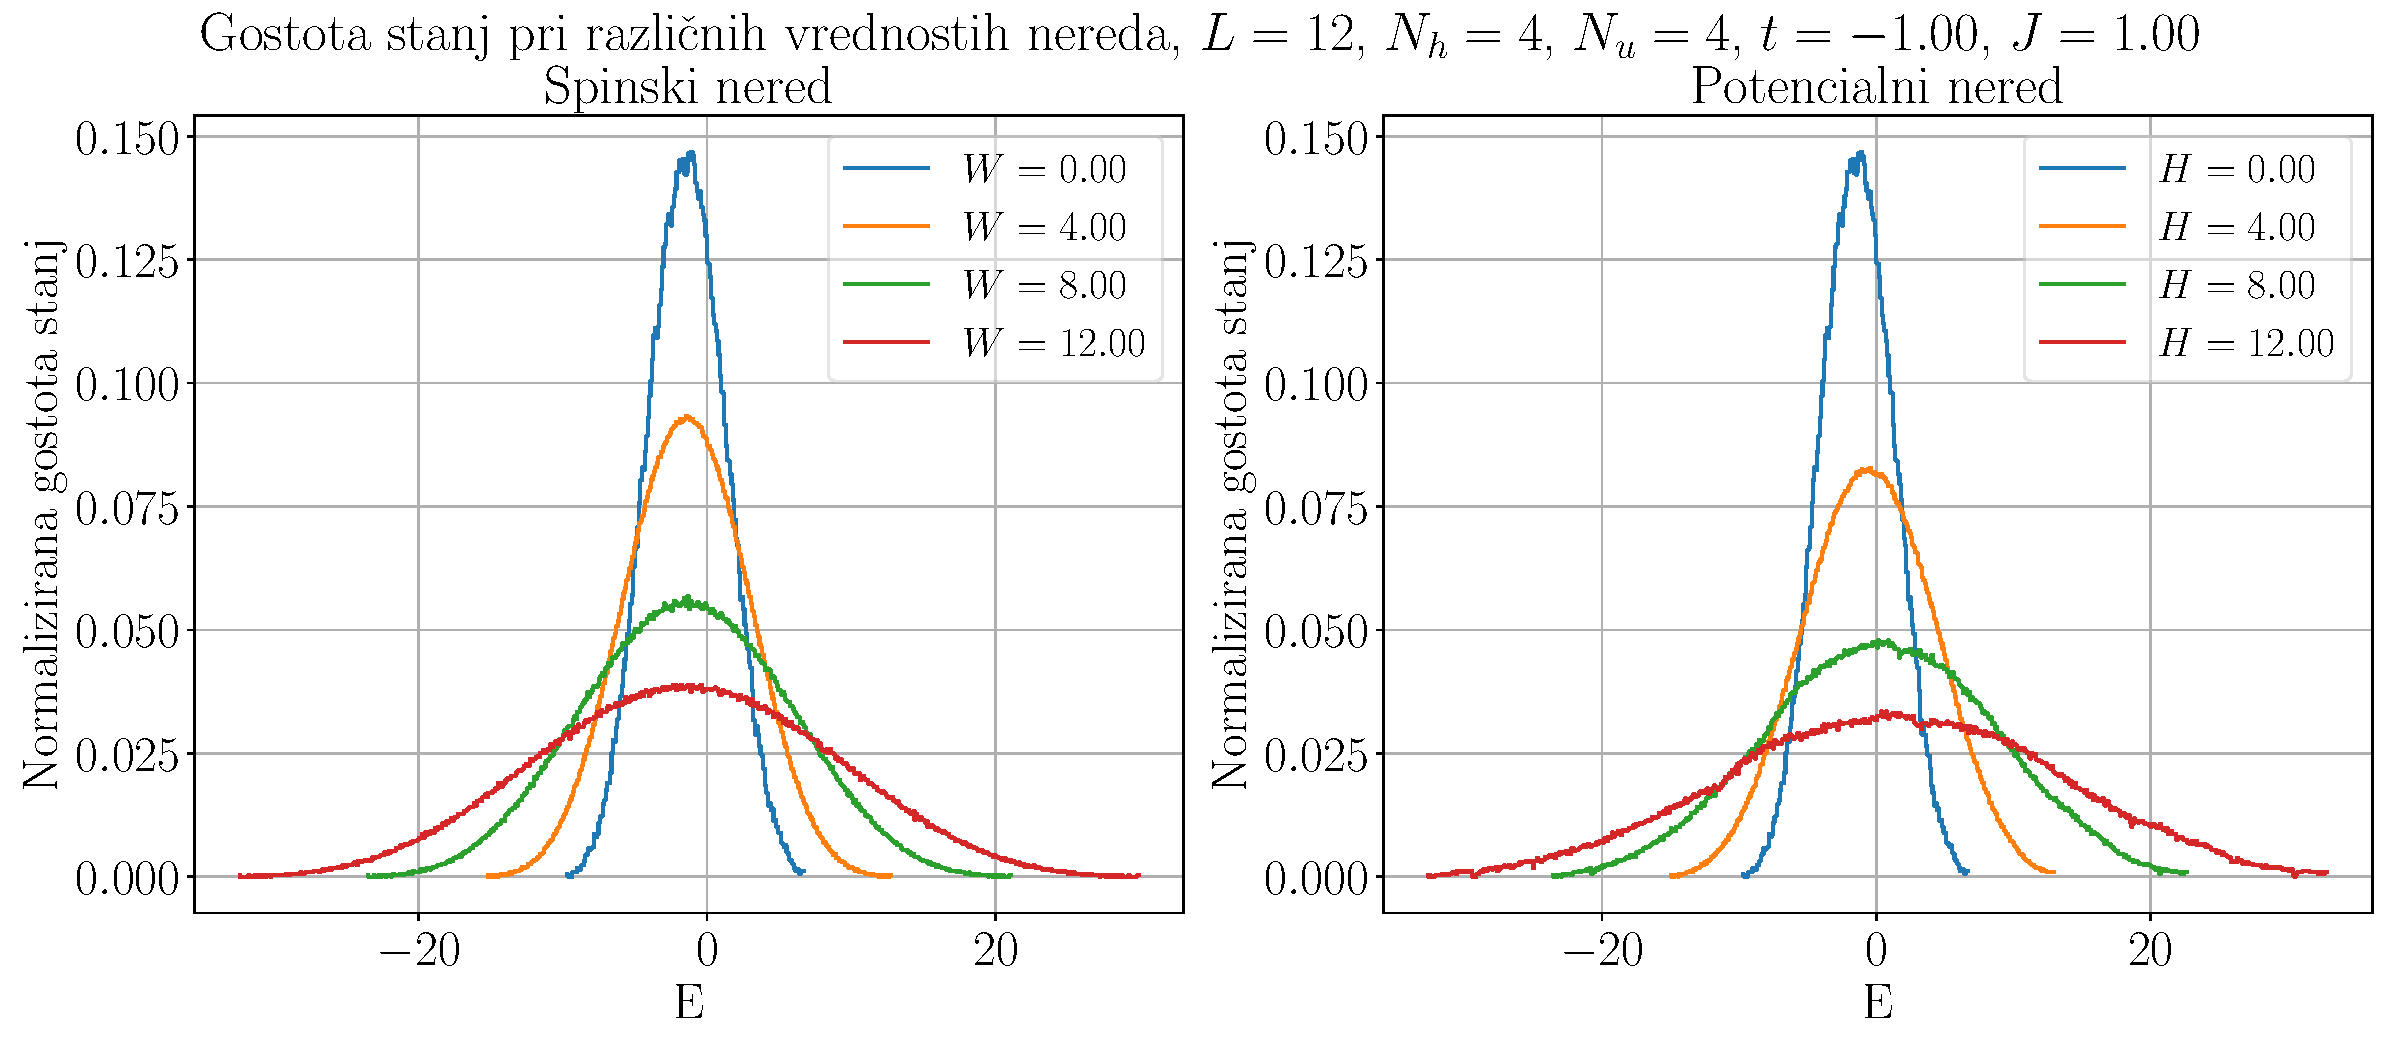
\includegraphics[width=1\textwidth]{DOS_spin_hole_disorder_12_4_4.pdf}}
\caption{Gostota stanj za primer s tretjinskim dopiranjem in spinskim oziroma potencialnim neredom. Oscilacij gostote stanj v primeru potencialnega nereda tokrat ne opazimo, saj pri dani spinski konfiguraciji vselej obstaja 495 možnih konfiguracij vrzeli. Posamezne naključne potencialne energije imajo v tem primeru le 70-kratno degeneracijo. }
\label{fig:DOS_spin_hole_disorder_12_4_4.pdf}
\end{figure}


V naslednjih dveh podpoglavjih razložim ključna koraka numerične implementacije obravnavanih metod, in sicer razgrnjenje spektra in lokalni zlom simetrije. 
\subsection{Razgrnjenje spektra}
Pred izračunom statistike za razmik med nivoji, podan z En. \eqref{eq:razmik}, izvedem \emph{razgrnjenje} spektra (ang. \emph{spectral unfolding})~\cite{abul2014unfolding}, s katerim povprečni razmik med nivoji fiksiram na enotsko vrednost. To omogoča medsebojno primerjavo statistike različnih spektrov, ki imajo sicer v splošnem kvantitativno različno gostoto stanj. Slednje je razvidno z grafov na Slikah~\ref{fig:Eigenstates_spin_hole_disorder_13_1_6.pdf} in~\ref{fig:DOS_spin_hole_disorder_13_1_6.pdf}, kjer sprememba parametra nereda znatno vpliva na obliko spektra in gostote stanj. Podobno na gostoto stanj pri enakih vrednostih modelskih parametrov vpliva tudi sprememba velikosti sistema, ki spremeni število stanj. \\\\
Po diagonalizaciji dobim spekter po velikosti urejenih lastnih vrednosti $E_i$ in definiram \emph{kumulativno število nivojev} $\tilde{N}(E)$ z energijo, manjšo od $E$, kot
\begin{equation}\label{eq:unfolding}
\tilde{N}(E)=\sum\limits_{E_i}\Theta(E_i-E).
\end{equation}
V odvisnosti $\tilde{N}(E_j)$ kjer je $j$ zaporedni indeks lastnega stanja, je razmik med zaporednimi nivoji po definiciji En. \eqref{eq:unfolding} enak 1. Diskretni kumulativni porazdelitvi $\tilde{N}(E_j)$ priredim polinomsko krivuljo $g(E_j)$ dovolj visoke stopnje, za kar v programskem jeziku \url{python} uporabim funkciji \url{polyfit} in \url{poly1d} iz knjižnice \url{numPy}. Namesto razmika med nivojema $E_n$ in $E_{n+1}$ v energijskem spektru tako spremljam razmik med nivojema prilagojenega polinoma $g(E_{n})$ in $g(E_{n+1})$. Vlogo razmika med sosednjimi nivoji $s$, podanega z En. \eqref{eq:razmik}, ima tako v mojih izračunih v resnici količina $\tilde{s}$, podana kot
$$
\tilde{s}_n=g(E_{n+1})-g(E_n).
$$
Razgrnitev spektra je potrebna pri izračunih statistike razmikov med sosednjimi nivoji (glej Sliko~\ref{fig:unfolding_demo_three_slo}), pri statistiki razmerij razmikov med sosednjimi nivoji $\tilde{r}$, ki jo podaja En. \eqref{eq:oganesyan_huse}, pa ne. V tem primeru je količina namreč že po definiciji omejena na interval med 0 in 1 in tako nanjo učinki velikosti sistema in spremenljive gostote stanj nimajo vpliva. Primer razgrnitve spektra je prikazan na Sliki~\ref{fig:unfolding_schematics}.
\begin{figure}[H]
\floatbox[{\capbeside\thisfloatsetup{capbesideposition={left,center},capbesidewidth=6.5cm}}]{figure}[\FBwidth]
{\caption{Primer razgrnitve spektra za sistem z $L=5$, $N_h=3$ in $N_u=1$, ki ima 20 stanj. Ker napovedi RMT dobro veljajo za stanja v središču spektra~\cite{d2016quantum}, poleg tega so stanja na robovih spektra občutljivejša na učinke končne velikosti sistema, v svojih izračunih v spektru vselej upoštevam le polovico stanj med prvim in zadnjim kvartilom vseh stanj, zato je na grafu prikazanih le 10 točk. Kot najprimernejša izbira za glajenje porazdelitve se kaže kar polinom stopnje 2, pri prevelikih vrednostih $n$ nastopijo težave s slabo pogojenostjo polinomov. }\label{fig:unfolding_schematics}}
{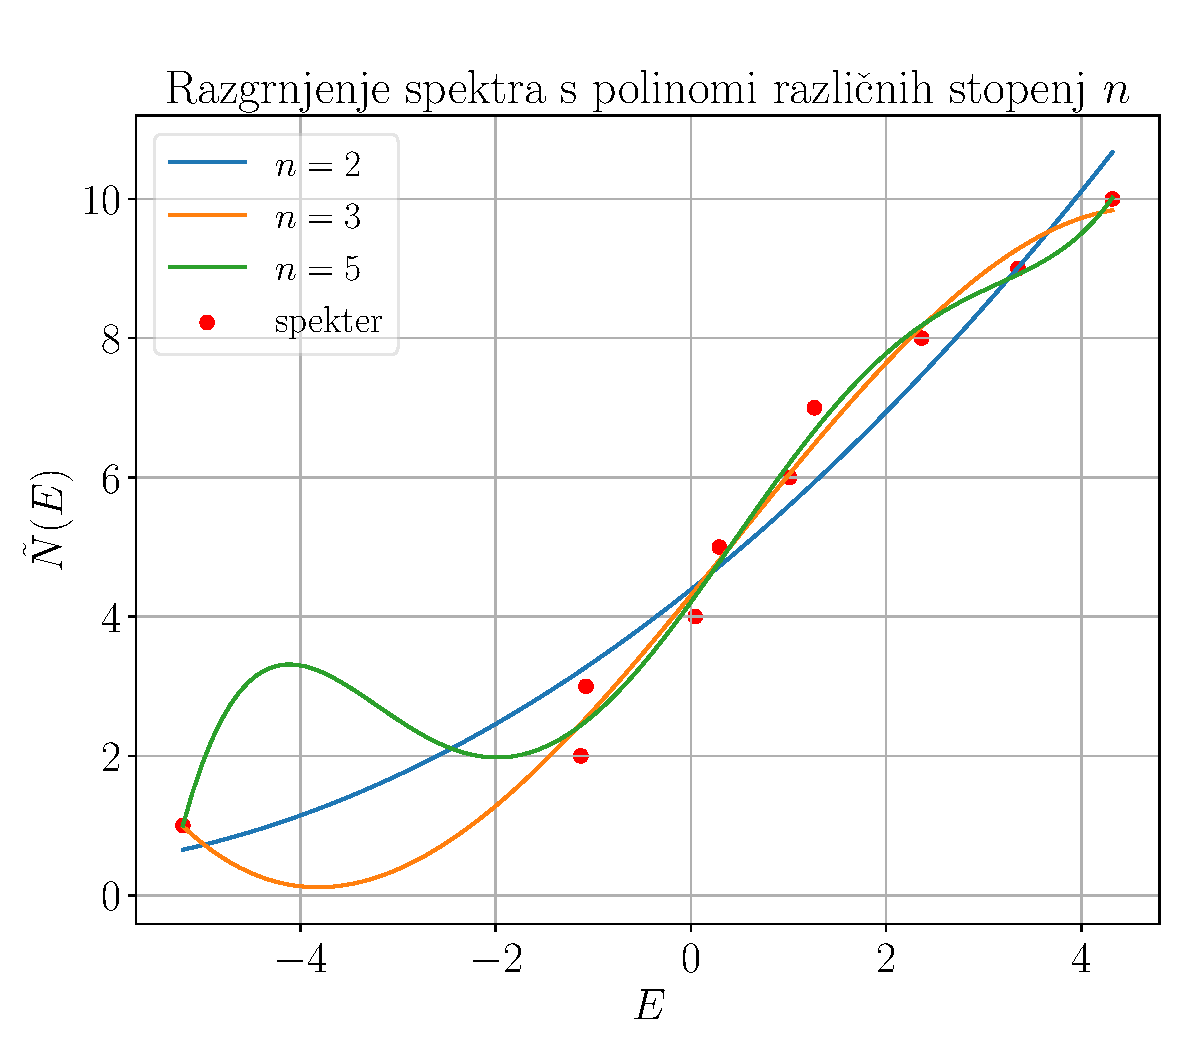
\includegraphics[width=0.55\textwidth]{unfolding_schematics.pdf}}
\end{figure}
\subsection{Lokalni zlom simetrije}
Obravnava katerekoli izmed do zdaj navedenih nivojskih statistik je smiselna samo v primeru, ko v spektru nimamo degeneracij, ki so posledica nezlomljenih simetrij hamiltonke. Za primerno analizo moramo torej bodisi na primeren način izbrati bazo sistema in spekter preučevati samo na enem izmed simetrijskih podprostorov hamiltonke bodisi moramo hamiltonki dodati šibko perturbacijo, ki zlomi simetrije, vendar bistveno ne spremeni energijske skale sistema. Sam pri svoji analizi uporabljam drugo možnost, in sicer hamiltonki dodam lokalna člena, ki se sklapljata s spinom oziroma z vrzelmi:
\begin{equation}\label{eq:sym_break_terms}
\hat{h}_\mathrm{spin}=W_\mathrm{sym}\hat{S}_1^z, \hspace{5mm} \hat{h}_\mathrm{hole}=H_\mathrm{sym}\hat{n}_L.
\end{equation}
Pri tem sta $W_\mathrm{sym}$ in $H_\mathrm{sym}$ parametra spinskega in vrzelnega zloma simetrije. Kolikšna mora biti njuna velikost, določim iz pogoja, da moram v ergodičnem režimu ob odsotnosti vsakršnega nereda za povprečje $\langle\tilde{r} \rangle$ dobiti vrednost $\langle\tilde{r}\rangle_\mathrm{GOE}=0.5307$. Rezultati analize zloma simetrije so prikazani na Sliki~\ref{fig:hole_spin_disorder_sym_break_13_1_6_slo}.

\begin{figure}[H]
\floatbox[{\capbeside\thisfloatsetup{capbesideposition={left,center},capbesidewidth=5cm}}]{figure}[\FBwidth]
{\caption{ Povprečna vrednost $\langle\tilde{r}\rangle$ ob odsotnosti vsakršnega nereda pri skupnem povečevanju parametrov $W_\mathrm{sym}$ in $H_\mathrm{sym}$. V kolikor so v spektru prisotne nezlomljene simetrije, potem statistika ob odsotnosti nereda ni dobro definirana in vrne napačen rezultat. Za vse prikazane velikosti sistema degeneracije učinkovito odpravi vrednost $W_\mathrm{sym}=H_\mathrm{sym}=0.5$, pri čemer vrednost z naraščajočim $L$ pada. Z rdečo in zeleno premico sta označeni vrednosti $\langle \tilde{r}\rangle_\mathrm{GOE}$ oziroma $\langle \tilde{r}\rangle_\mathrm{Poisson}$. }\label{fig:hole_spin_disorder_sym_break_13_1_6_slo}}
{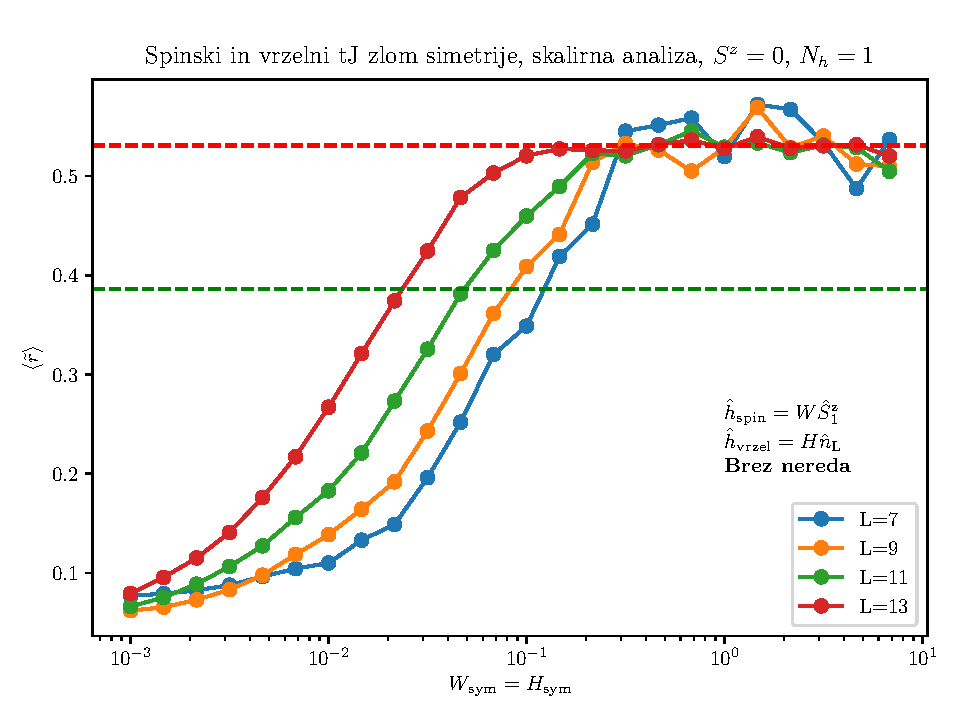
\includegraphics[width=0.7\textwidth]{hole_spin_disorder_sym_break_13_1_6_slo.pdf}}
\end{figure}
V kolikor simetrij ne odpravimo, bo porazdelitev nivojske statistike v splošnem konvolucija nivojskih statistik za posamezne simetrijske sektorje hamiltonke. Zaradi morebitnega prekrivanja energijskih nivojev iz različnih simetrijskih sektorjev odboj med nivoji v ergodični fazi v tem primeru ni tako zaznaven. V statistiki razmikov med sosednjimi nivoji to opazimo kot prisotnost neničelne vrednosti $p(s=0)$, povprečje $\langle \tilde{r}\rangle$ pa je manjše, kot bi sicer pričakovali v ergodičnem režimu. 

\subsection{Rezultati}
Z dodanim lokalnim zlomom simetrije so nivojske statistike dobro definirane tudi v primeru odsotnosti vsakršnega nereda - pri $H=W=0$ ima $\langle \tilde{r}\rangle$ vrednost v bližini  $\langle \tilde{r}\rangle_\mathrm{GOE}$. Na Slikah~\ref{fig:double_plot_disorder_sym_break_13_1_6_slo} in~\ref{fig:double_plot_disorder_sym_break_12_4_4_slo} so prikazani rezultati skalirne analize za odvisnost $\langle \tilde{r}\rangle$ v primeru dopiranja z eno vrzeljo in v primeru tretjinskega dopiranja. Na Slikah~\ref{fig:r_density_11_1_5} in~\ref{fig:r_density_9_3_3} sta prikazana še primera sprehodov po prostoru parametrov $H$ in $W$ pri izračunu $\langle \tilde{r} \rangle$.
 \begin{figure}[H]
\centering{
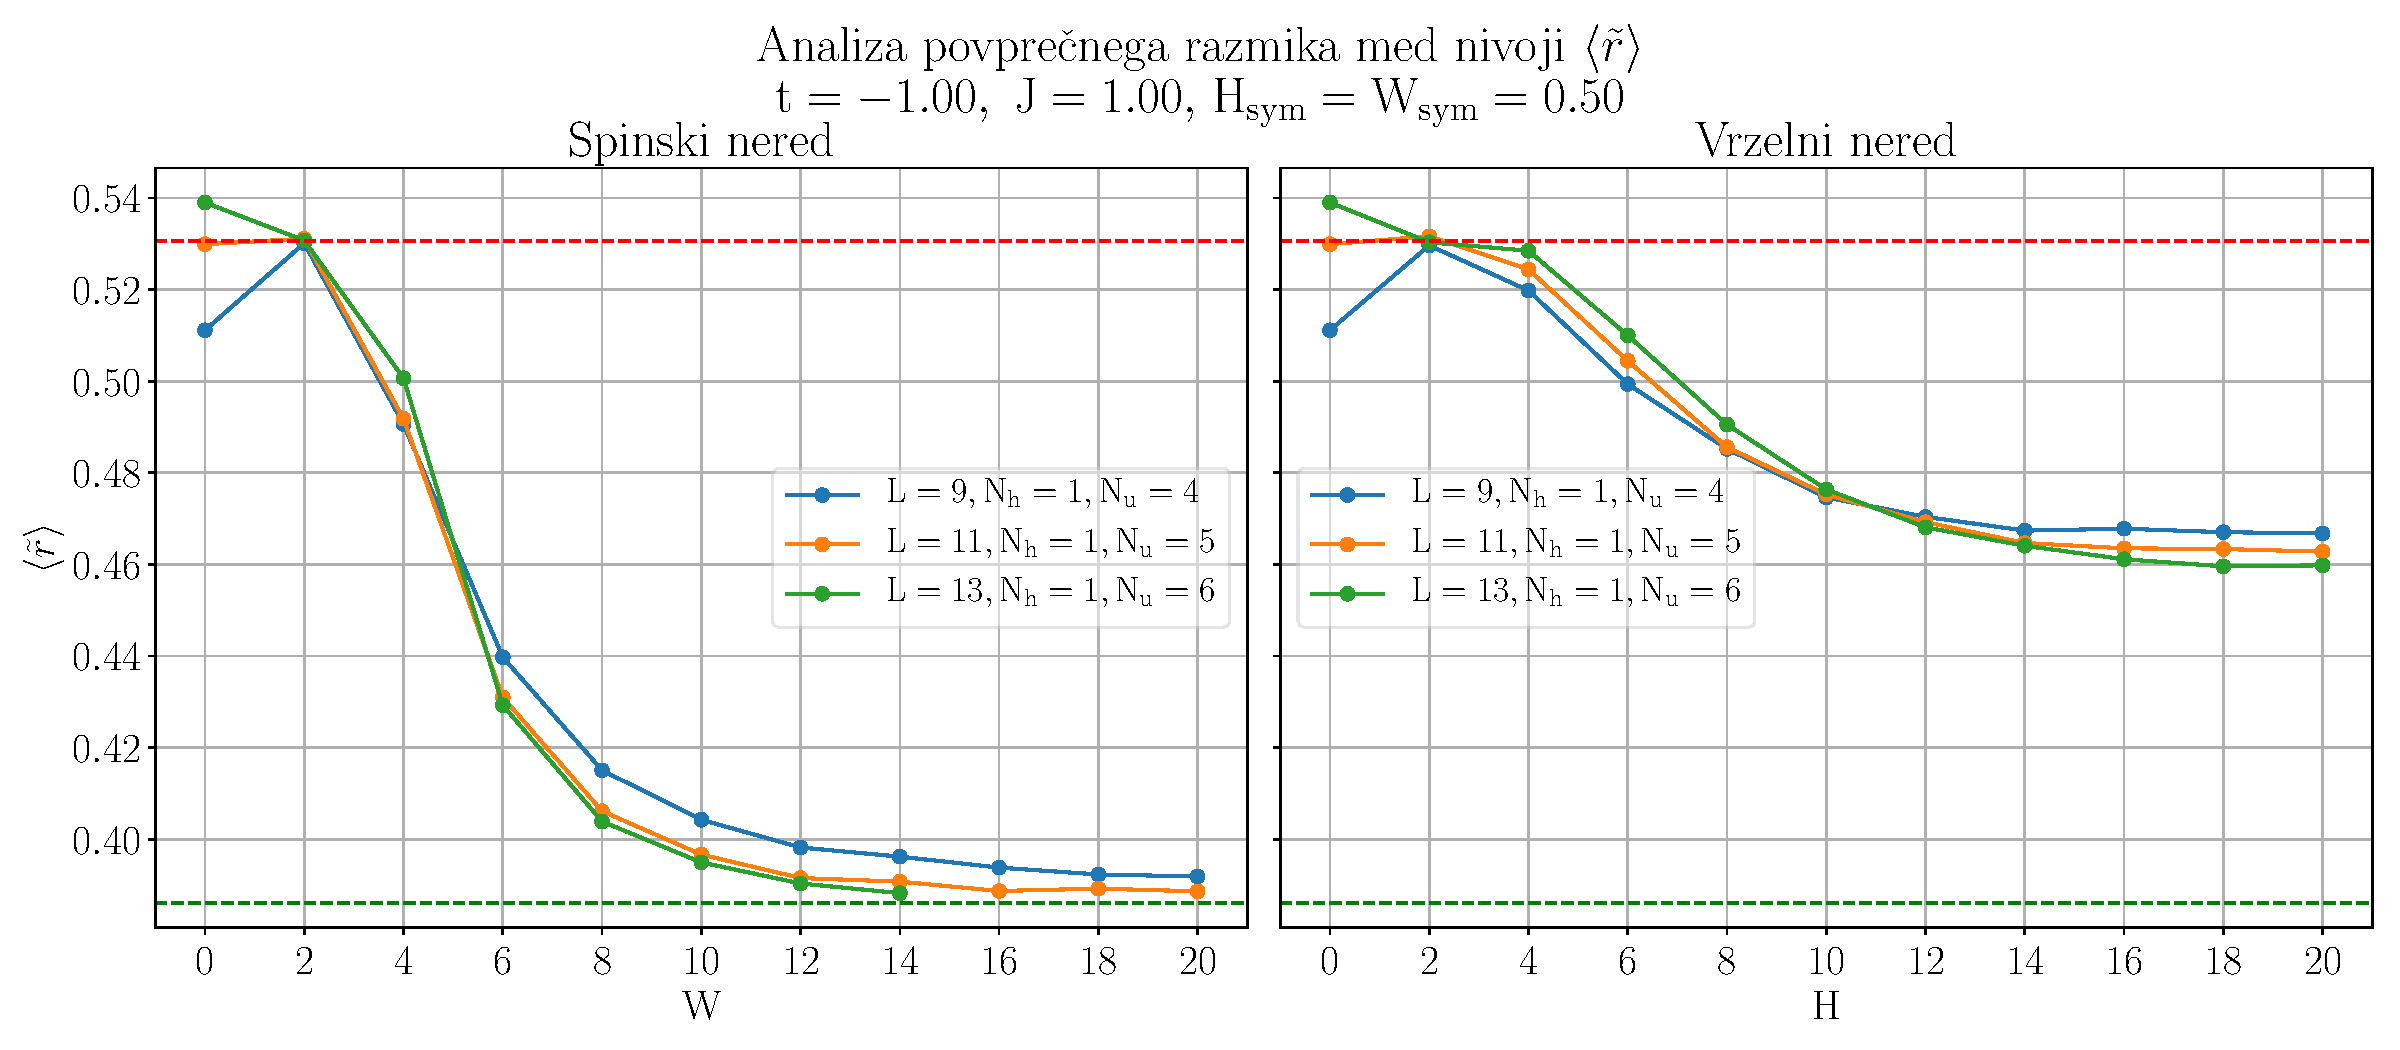
\includegraphics[width=1\textwidth]{double_plot_disorder_sym_break_13_1_6_slo.pdf}}
\caption{Zaradi majhnega števila primernih sistemov (sistemi z $L<9$ imajo premalo stanj za primerno statistiko, sistemi z $L>15$ so preveliki za naše računske zmogljivosti) je skalirna analiza, ki bi omogočila ekstrapolacijo rezultatov proti termodinamski limiti neskončnega sistema, razmeroma zahtevna če ne nemogoča naloga. Kljub temu lahko sklepamo, da v primeru ene vrzeli povečevanje spinskega nereda vodi do prehoda v MBL režim, medtem ko nered, ki se sklaplja z vrzelmi, ne pripelje do večdelčne lokalizacije. Nekoliko presenetljivo se zdi, da se v primeru vrzelnega nereda vrednost $\langle \tilde{r}\rangle$ z naraščanjem $L$ pomika navzdol, saj bi v termodinamski limiti pričakoval, da bo prispevek nereda na eni vrzeli zanemarljivo majhen. }
\label{fig:double_plot_disorder_sym_break_13_1_6_slo}
\end{figure} 
\begin{figure}[H]
\centering{
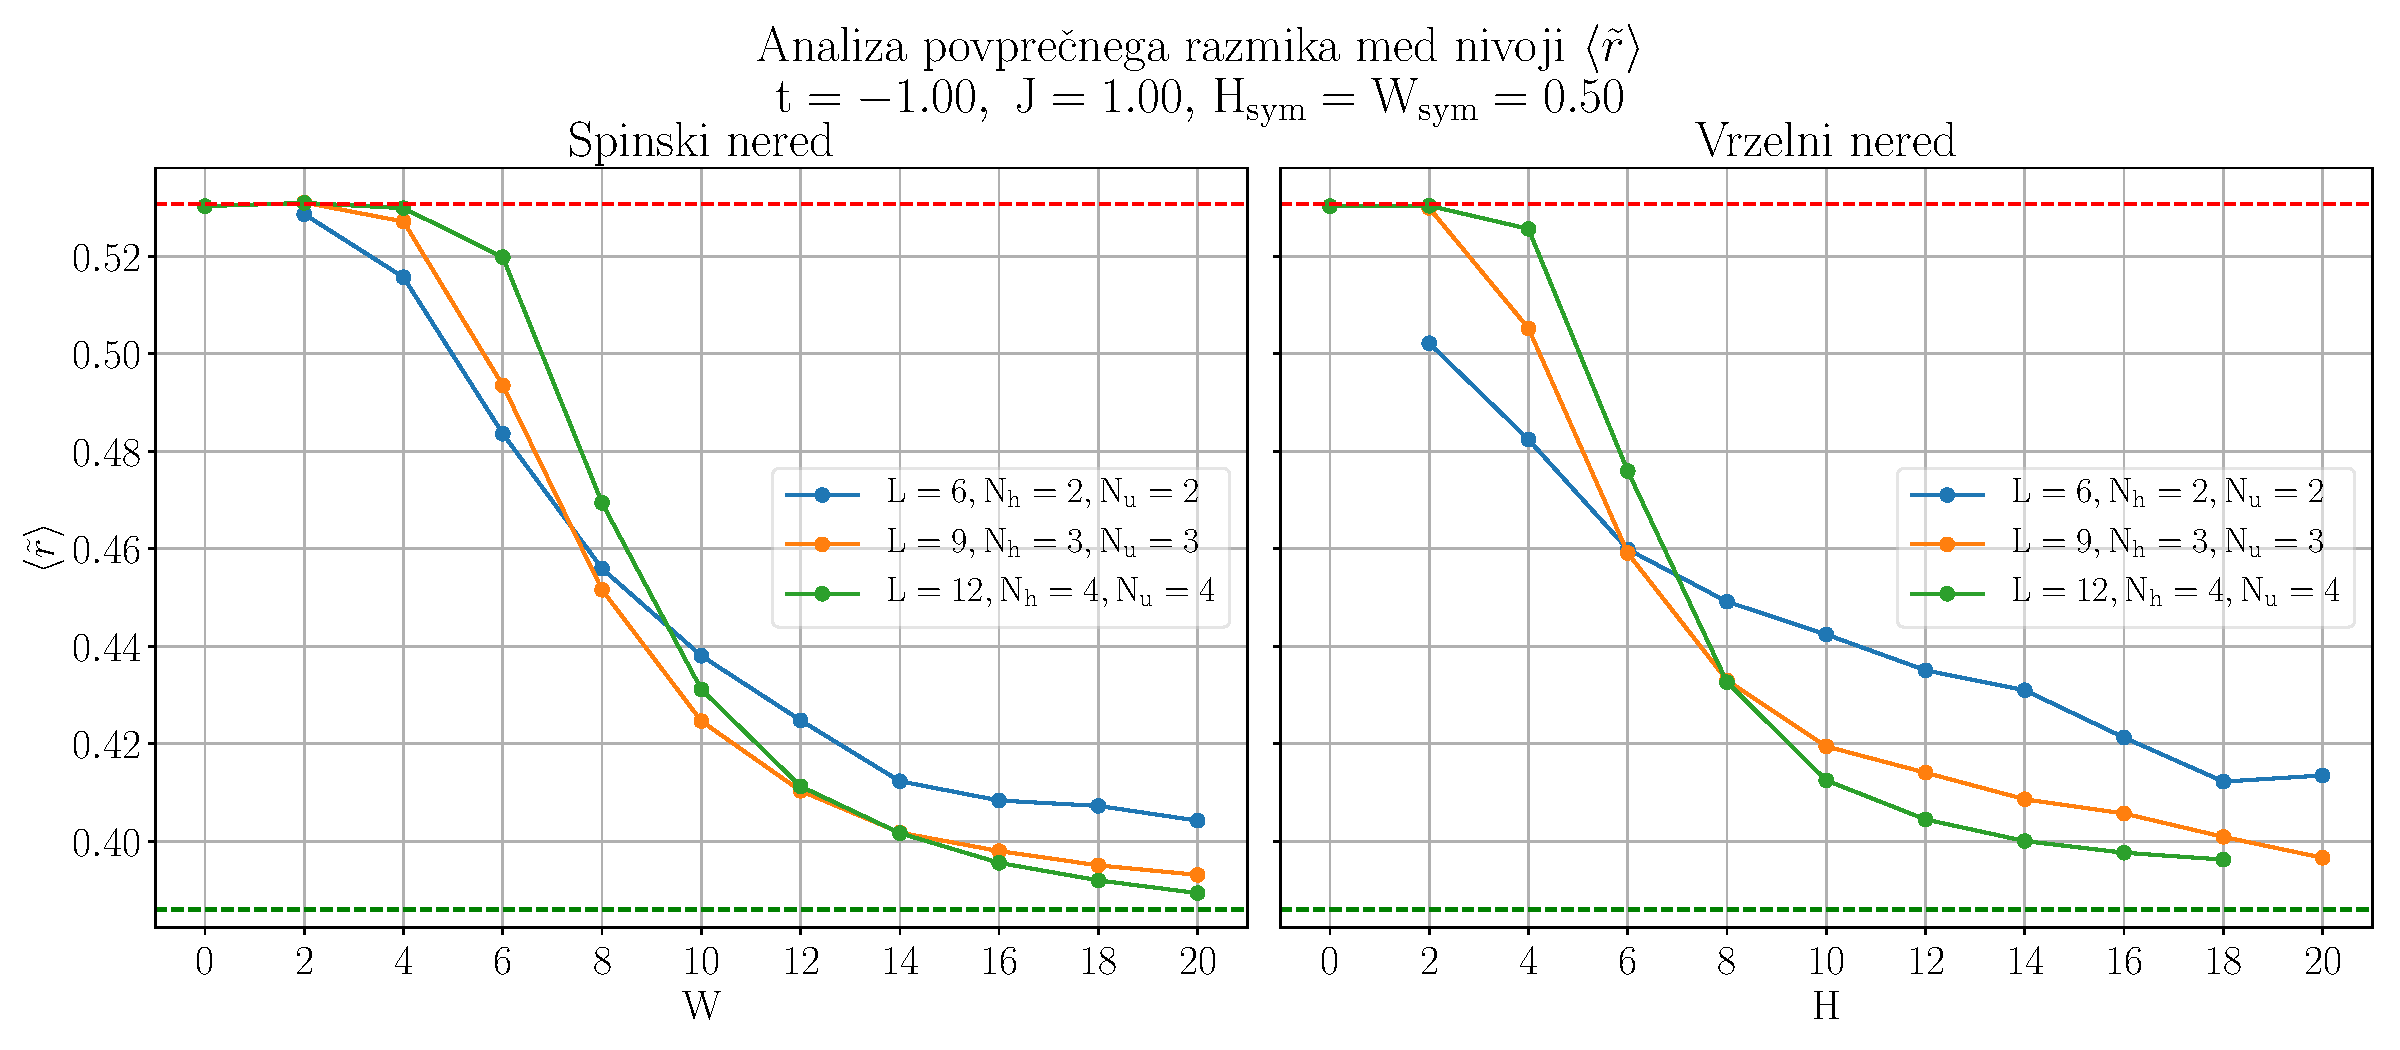
\includegraphics[width=1\textwidth]{double_plot_disorder_sym_break_12_4_4_slo.pdf}}
\caption{Pri tretjinskem dopiranju se zdi, da lahko oba tipa nereda pripeljeta do večdelčne lokalizacije. Krivulja za $L=6$ je statistično nepomembna, saj ima ta sistem zgolj 90 stanj, kar je očitno premalo za zanesljivo statistiko. Fluktuacije povprečnih količin namreč padajo z velikostjo sistema. Zaradi omejenega števila sistemov, ki so na voljo za preučevanje, je skalirna analiza, s katero bi določil, kje v termodinamski limiti neskončnega sistema pride do prehoda med MBL in ergodičnim sistemom, otežena.  }
\label{fig:double_plot_disorder_sym_break_12_4_4_slo}
\end{figure}
\begin{figure}[H]
\floatbox[{\capbeside\thisfloatsetup{capbesideposition={left,center},capbesidewidth=5cm}}]{figure}[\FBwidth]
{\caption{Vrednosti $\langle \tilde{r}\rangle$ v odvisnosti od $H$ in $W$ za primer dopiranja z eno vrzeljo pri velikosti sistema $L=11$ ter povprečenjem po 300 naključnih realizacijah za obe vrsti nereda. Modra oz. temnejši toni označuje(jo) MBL režim, rumeni in zeleni odtenki pa pomenijo ergodičnost. Pri majhnem spinskem neredu opazimo, da še tako velike vrednosti $H$ ne pripeljejo do lokalizacije. }\label{fig:r_density_11_1_5}}
{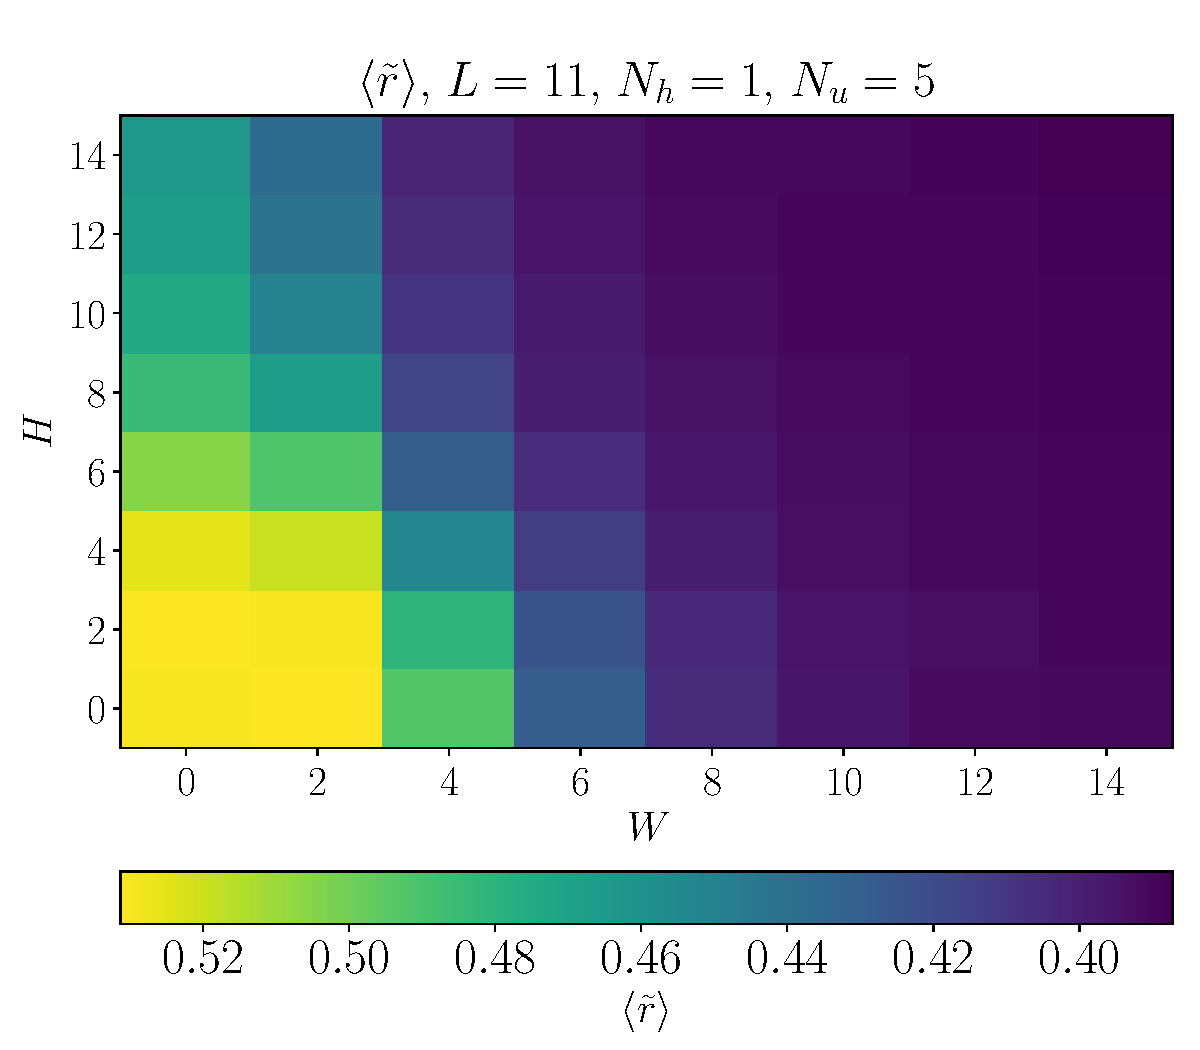
\includegraphics[width=0.6\textwidth]{r_density_11_1_5.pdf}}
\end{figure}
\begin{figure}[H]
\floatbox[{\capbeside\thisfloatsetup{capbesideposition={left,center},capbesidewidth=5cm}}]{figure}[\FBwidth]
{\caption{Sprehod po prostoru parametrov $H$ in $W$ pri izračunu $\langle \tilde{r}\rangle$ še za primer tretjinskega dopiranja in ponovno povprečenja po 300 naključnih realizacijah nereda, $L=9$. Spreminjanje obeh parametrov vodi do lokalizacije, pri čemer se zdi vloga obeh parametrov dokaj enakovredna. }\label{fig:r_density_9_3_3}}
{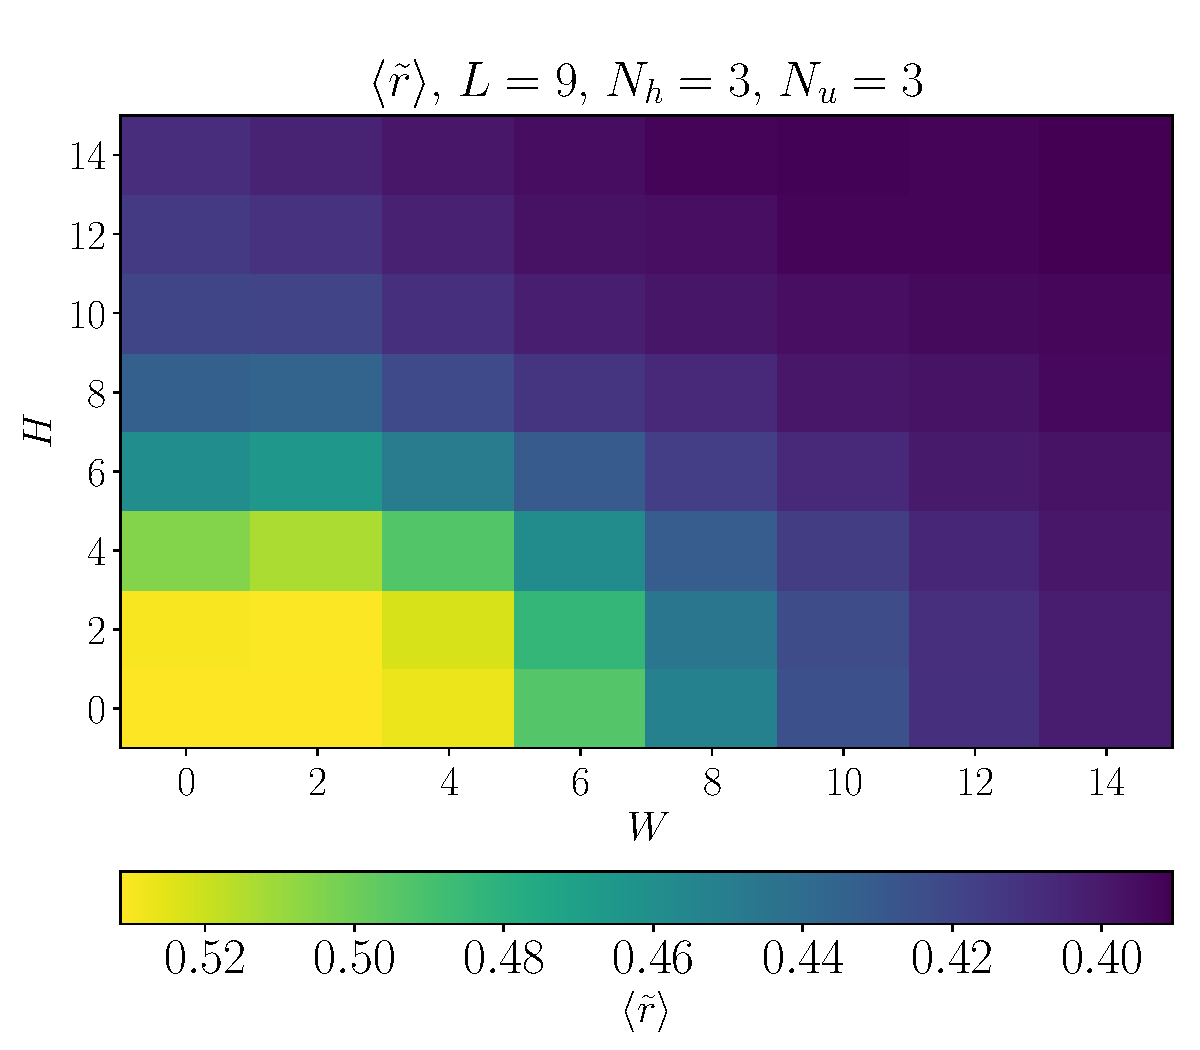
\includegraphics[width=0.6\textwidth]{r_density_9_3_3.pdf}}
\end{figure}
\section{Zaključek}
V zaključni nalogi sem predstavil numerično implementacijo izračuna spektralnih statistik porazdelitve razmikov med sosednjimi nivoji v energijskem spektru in izračun povprečnega razmerja razmikov zaporednih nivojev za model t-J. Področje večdelčne lokalizacije v sistemih interagirajočih delcev z dodanim neredom  je trenutno popularna tema na področju raziskav v fiziki koreliranih sistemov, v katerih nered igra ključno vlogo pri prehodu iz izolatorskega v prevodni režim.\\\\
Izračunane vrednosti parametrov $W$ in $H$, pri katerih v poročilu predstavljene statistike napovedo nastop prehoda iz ergodičnega v MBL režim, so večje od vrednosti, izračunanih s komplementarnimi študijami dinamike časovnega razvoja netipičnih začetnih porazdelitev~\cite{lemut2017complete} za isti sistem ob prisotnosti ene vrzeli, vendar velja pri medsebojni primerjavi rezultatov obeh metod previdnost: v poročilu predstavljeni statistiki obravnavata zgolj korelacije med sosednjimi energijskimi nivoji, upoštevata torej zgolj najmanjše energijske skale v sistemu.
 Posledično na podlagi študij sosednjih energijskih nivojev izluščimo zgolj informacije o dogajanju v sistemu na najdaljših časovnih skalah, ki jih s časovno propagacijo začetnih stanj zaradi efektov končnih velikosti sistema tipično ne moremo doseči. Zaradi majhnega števila sistemov, s katerimi bi lahko preveril skaliranje rezultatov v termodinamski limiti, ne morem z gotovostjo locirati kritičnih parametrov faznega prehoda. Medtem ko spinski nered pri dovolj velikih vrednostih $W$ v vseh obravnavanih primerih povzroči lokalizacijo, je pri potencialnem neredu pomembna tudi vloga dopiranja z vrzelmi - lokalizacija nastopi v primeru tretjinskega dopiranja, pri dopiranju z eno vrzeljo pa ne. 
%\begin{thebibliography}{9}
%\bibitem{NumRec}
%W. H. Press, \emph{Numerical Recipes in C}, Cambridge: Cambridge University Press, (1992).
%
%\end{thebibliography}
\bibliographystyle{fmf-sl}
\bibliography{literatura}

% \printindex


\end{document}


